\chapter{Multiscale turbulence measurements}
\label{ch:TurbulenceMeasurements}
The development of a first-principles understanding
of turbulent transport in a tokamak
is a long-standing goal of the fusion community.
Such a model would allow accurate design and optimization of a tokamak.
Before such a model is accepted, however,
it must be validated against experimental measurements.
Ideally, this validation should be multi-tiered,
with the model accurately and robustly reproducing
experimental observations at all scales,
from macroscopic parameters such as the turbulent heat flux to
the details of the turbulent spectrum
(e.g.\ power spectral densities, cross phases, nonlinear couplings, etc.).

Along these lines,
this chapter presents measurements of electron-density turbulence
made over a wide spatiotemporal bandwidth
during a recent \diiid\space experiment.
Section~\ref{sec:TurbulenceMeasurements:Background}
begins with a brief overview of the drift-wave turbulence
often observed in tokamak plasmas,
emphasizing recent results
from realistic multiscale simulations
\cite{howard_pp14, howard_nf16, howard_pp16, howard_ppcf18, holland_nf17}.
Section~\ref{sec:TurbulenceMeasurements:ExperimentalConditions}
then describes the recent \diiid\space experiment,
which was designed to probe the multiscale nature
of plasma turbulence.
As such, this experiment presents an ideal opportunity
for multiscale turbulence investigations
with the combined PCI-interferometer.
Next, Section~\ref{sec:TurbulenceMeasurements:Measurements}
details the measurements from the combined PCI-interferometer.
Numerous turbulent branches are observed.
In particular, the interferometer measures
a low-$k$ electromagnetic mode driven unstable by collisionality,
properties consistent with the micro-tearing mode (MTM), and
the PCI measures a wavenumber spectrum
that exhibits distinct flattening
when increasing the electron-scale turbulent drive
relative to the ion-scale turbulent drive,
reminiscent of results
from realistic multiscale gyrokinetic simulations~\cite{howard_pp16}.
Finally, to aid the interpretation of these measurements,
linear-stability analysis and quasilinear-transport modeling
are performed with the TGLF code
in Section~\ref{sec:TurbulenceMeasurements:Modeling}, and
qualitative agreement with the PCI-measured wavenumber spectrum
is obtained.


\section{Overview of drift-wave turbulence}
\label{sec:TurbulenceMeasurements:Background}
The radial transport of particles, heat, and momentum in a tokamak plasma is
often larger than that predicted by collisional (i.e.\ neoclassical) theory.
There is strong theoretical and experimental evidence
that this ``anomalous'' transport
results from drift-wave turbulence
driven by the free energy in the plasma gradients
\cite{horton_drift_waves,tynan_ppcf09}.
This turbulence can be characterized by
its driving gradients,
its spatiotemporal characteristics,
the role of trapped particles, and
whether or not it is electrostatic
(as opposed to electromagnetic).

The plasma gradients are often quantified in terms of scale lengths.
The scale length of quantity $x$ is defined as
$L_x = x / \nabla x = (\nabla \ln x)^{-1}$.
Smaller values of $|L_x|$ indicate
more rapid spatial variation
(i.e.\ steeper gradient) of quantity $x$.
Thus, the free energy in profile $x$ increases with
the inverse scale length $1 / L_x$.
For theoretical analysis,
it is conventional to normalize $L_x$
to a relevant length in the system under study;
below, scale lengths are normalized
to the tokamak minor radius $a$,
which is appropriate for studies of radial transport.
Thus, the drive for instability is quantified
by the normalized inverse scale length $a / L_x$.
The ratio of density scale length to temperature scale length
$\eta_j = L_{n_j} / L_{T_j}$ for species $j$
is an additional dimensionless parameter
that is often used for instability characterization.

Due to the relatively large size of its eddies,
ion-scale ($k_{\theta} \rho_s < 1$) turbulence is often considered
to be the most detrimental to confinement.
Here, $k_{\theta}$ is a typical poloidal wavenumber of the turbulent mode,
$\rho_s = c_s / \Omega_i$ is the ion gyroradius
evaluated at the ion sound speed,
$c_s = (T_e / m_i)^{1/2}$ is the ion sound speed, and
$\Omega_i = e B / m_i$ is the ion angular cyclotron frequency.
The temporal ordering of ion-scale turbulence is usually expressed as
$k_{||} \text{v}_{ti} \ll \omega \ll k_{||} \text{v}_{te}$
\cite[Sec.~8.3]{wesson},
where $\omega$ is the angular frequency of the instability,
$k_{||}$ is the instability wavenumber parallel to the magnetic field, and
$\text{v}_{tj}$ is the thermal speed of species $j$;
thus, the electrons respond rapidly (approximately adiabatically)
to the electrostatic-potential fluctuations
of the instability.
Typically, trapped-ion dynamics make insignificant contributions
to ion-scale drift-wave turbulence in tokamak plasmas
\cite[Sec.~IV.E]{horton_drift_waves};
passing-particle dynamics, however, are significant and
produce the $\eta_i$ mode, which
is driven linearly unstable
above a critical value of $\eta_i$ ($\eta_i^{\text{crit}} \sim 1$)
\cite[Sec.~8.3]{wesson} and
peaks about $k_{\theta} \rho_s \sim 0.3$~\cite[Sec.~1.2.1]{tynan_ppcf09}.
For sufficiently flat density profiles
($a / L_{n_i} \lesssim 1$,
which is valid across most of the radial domain
for the plasmas considered in this work),
the toroidal $\eta_i$ mode has a critical value
$\eta_{i}^{\text{crit}} = \eta_{i}^{\text{crit}}(L_{T_i})$,
independent of $L_{n_i}$;
for this reason, the $\eta_i$ mode is
also often referred to as
the ion temperature gradient (ITG) mode~\cite[Sec.8.3]{wesson},
driven more unstable by larger values of $a / L_{T_i}$.

Despite having much smaller eddy size
than its ion-scale counterparts,
electron-scale ($k_{\theta} \rho_s > 1$) turbulence
may still make large contributions to plasma transport.
Of particular importance
is the electron temperature gradient (ETG) mode.
The physics of the ETG is comparable to that of the ITG,
with the roles of the ions and electrons reversed.
(Here, the ion response is approximately adiabatic
because the electrostatic potential fluctuations
occur on spatial scales much smaller than the ion gyroradius
\cite[Sec.~2.3.4.2]{fusion_physics_iaea}).
As the name suggests,
the ETG is driven more unstable by larger values of $a / L_{T_e}$
\cite[Sec.~8.3]{wesson}.
Relative to the ITG,
the ETG spatial scales in a $T_e \sim T_i$ plasma
are reduced by the square root
of the electron-to-ion mass ratio
$(m_e / m_i)^{1/2} \approx 60$ such that
the ETG peaks at $k_{\theta} \rho_s \sim 20$
in a deuterium plasma.
While electron-scale simulations have long shown that the ETG
may be capable of forming radially elongated ``streamers''
\cite{dorland_prl00}
capable of driving experimentally relevant electron heat transport
\cite{jenko_prl02},
it was unknown whether or not
such streamers would survive
in the presence of ion-scale turbulence,
as self-consistently and simultaneously simulating
both ion- and electron-scale turbulence with realistic mass ratios
was computationally intractable until very recently.

By exploiting the latest advances in high-performance computing,
Howard \emph{et al.} have performed
multiscale gyrokinetic simulations
with realistic mass ratios
for both L-mode~\cite{howard_pp14, howard_nf16, howard_pp16} and
H-mode plasmas~\cite{howard_ppcf18, holland_nf17}.
Indeed, under certain realistic conditions,
ETG streamers are predicted
to coexist with the ITG and
to drive empirically relevant levels
of electron heat flux~\cite{howard_pp14}.
Local and non-local energy cascades
between the ion and electron scales
are also predicted~\cite{howard_nf16},
indicating the importance of cross-scale coupling.
This cross-scale coupling becomes stronger
as the ETG drive $a / L_{T_e}$ increases
relative to the ITG drive $a / L_{T_i}$
\cite{howard_pp16}.
Further, flattening of the wavenumber spectrum
is predicted to be a tell-tale signature
of this enhanced cross-scale coupling~\cite{howard_pp16}.

Seeking empirical validation of these predictions,
Howard \emph{et al.} recently performed an experiment at \diiid\space
to alter the local $a / L_{T_e}$ and $a / L_{T_i}$.
The reference discharge for this experiment,
\diiid\space shot $153523$,
was selected because multiscale gyrokinetic simulations
indicate that its turbulent transport
is intrinsically multiscale in nature~\cite{holland_nf17}.
The experimental conditions are discussed
in Section~\ref{sec:TurbulenceMeasurements:ExperimentalConditions}, and
the combined PCI-interferometer measurements
of the resulting electron-density fluctuations are presented
in Section~\ref{sec:TurbulenceMeasurements:Measurements}.
To aid the interpretation of these measurements,
linear-stability analysis and quasilinear-transport modeling
is performed in Section~\ref{sec:TurbulenceMeasurements:Modeling}.
While the plasmas simulated in the above multiscale work
were ITG-ETG dominant,
Sections~\ref{sec:TurbulenceMeasurements:Measurements} and
~\ref{sec:TurbulenceMeasurements:Modeling}
indicate the presence of additional modes;
the basic properties of candidate modes
consistent with these observations
are briefly reviewed below.

The linear-stability analysis performed in
Section~\ref{sec:TurbulenceMeasurements:Modeling}
indicates the presence of
a mid-$k$ ($0.5 \lesssim k_{\theta} \rho_s \lesssim 5$) electron mode.
The mode is destabilized with
increasing $a / L_{T_e}$ (and decreasing $a / L_{T_i}$).
It is conceivable that this mode is
the trapped electron mode (TEM).
In contrast to the passing-particle dynamics of the ITG and ETG,
trapped-electron dynamics destabilize the TEM~\cite[Sec.~8.4]{wesson}.
Trapped particles effectively average out their parallel velocities
over a bounce period, but
they also spend most of their time
in regions of bad magnetic curvature,
producing stability characteristics
not unlike those seen in a magnetic mirror~\cite[Sec.~8.4]{wesson}.
Of course, trapped-particle dynamics
will only be important if
trapped particles are able to execute one or more bounce orbits
before being detrapped by collisions.
Thus, the TEM requires that most of the trapped electrons
are in the banana collisionality regime
($\nu_e^* < 1$)~\cite[Sec.~2.3.4.3]{fusion_physics_iaea}.
The spatiotemporal aspects of the TEM are characterized by
$k_{\theta} \rho_s \sim 1$ and
$\omega \sim \omega_{*e}$~\cite[Sec.~2.3.1]{fusion_physics_iaea},
where $\omega_{*e} = -k_{\theta} T_e (dn_e / dr) / (e B n_e)$
is the electron diamagnetic frequency~\cite[8.2]{wesson} and
the other parameters were introduced in the above ITG discussion.
(Note that $\omega_{*e}$ is derived from considerations
of the adiabatic electron response along the magnetic field,
which corresponds to the parallel electron temperature $T_{e,||}$;
however, in an isotropic temperature distribution,
$T_{e,||} = T_{e,\perp} = T_e$).
Both $a / L_{T_e}$ and $a / L_{n_e}$
provide free energy to the TEM~\cite[Sec.~2.3.1]{fusion_physics_iaea}.

Finally, Section~\ref{sec:TurbulenceMeasurements:Measurements}
identifies a low-$k$ ($k_R < \SI{1.5}{\per\centi\meter}$)
electromagnetic mode driven unstable by collisionality.
These properties are consistent with
the micro-tearing mode (MTM)~\cite[Sec.~8.5]{wesson},
which was predicted to be marginally unstable
for $k_y \rho_s \sim 0.2$
in this experiment's reference discharge~\cite{holland_nf17}.
While the ITG, ETG, and TEM are electrostatic,
the MTM is electromagnetic and
can produce small-scale magnetic islands.
Relative to conventional, macroscopic tearing modes,
the MTM has short wavelength and
high poloidal mode number $m$~\cite[Sec.~8.5]{wesson}.
Tearing-mode linear stability is often quantified by $\Delta'$,
a parameter derived from resistive MHD~\cite[Sec.~7.3]{wesson};
for the large poloidal mode number of the MTM,
the resulting $\Delta'$ predicts stability.
However, resistive MHD is an inadequate model for the MTM, and
both kinetic and nonlinear effects can compete with $\Delta'$
to destabilize the MTM in the presence of finite $\eta_e$
(i.e.\ finite electron temperature gradient).
Importantly, via kinetic effects, the MTM is unstable
at ``moderate'' $\nu_{ei} / \omega_{*e}$, where
$\nu_{ei}$ is the electron-ion collision frequency and
$\omega_{*e}$ is the electron diamagnetic frequency~\cite[Sec.~8.5]{wesson}.


\section{Experimental conditions}
\label{sec:TurbulenceMeasurements:ExperimentalConditions}
The experiment was run in the ITER-similar shape,
with aspect ratio, elongation, and triangularity
all closely matched to those of the ITER-baseline scenario
\cite[Sec.~13.5 \& 13.6]{wesson}.
The on-axis toroidal field $B_T = \SI{-1.7}{\tesla}$ and
plasma current $I_p = \SI{1.3}{\mega\ampere}$
produced $q_{95} = 3.15$,
where $q_{95}$ is the average value
of the safety factor $q$~\cite[Sec.~3.4]{wesson}
over the surface that encloses $95\%$
of the poloidal flux within the last-closed flux surface.
Neutral beam injection (NBI)~\cite[Sec.~5.3-5.5]{wesson}
was performed with feedback to maintain
$\beta_N = 1.9$, where
$\beta_N$ is the normalized plasma pressure~\cite[Sec.~6.18]{wesson}.
In order to suppress core MHD,
an average NBI torque of approximately $\SI{1.5}{\newton \meter}$
was injected into the plasma;
note that this is approximately four times larger than
the projected ITER-equivalent torque~\cite{garofalo_nf11}.
In order to alter the local electron-scale and ion-scale drives,
the electron cyclotron resonance heating (ECH)~\cite[Sec.~5.10]{wesson}
location was scanned between $\rho = 0.5$ and $\rho = 0.8$,
where $\rho$ is the square root of the normalized toroidal flux
(which scales as $r / a$, with
$r$ being the minor-radial coordinate and
$a$ being the minor radius of the plasma).
Intra-shot scans of the ECH location
were plagued with core MHD, so
only shot-to-shot, MHD-free scans of the ECH location
are considered here.
The line-averaged density was
$\bar{n}_e = \SI{5.2e19}{\per\meter\cubed}$.
Impurities were removed from the plasma
by both large and small edge localized modes (ELMs)~\cite[Sec.~7.17]{wesson}.
The time histories of several actuators and plasma parameters
are shown in Figure~\ref{fig:TurbulenceMeasurements:traces}.
Note that multiscale gyrokinetic simulations
of this experiment's reference discharge,
\diiid\space shot $153523$ with ECH at $\rho = 0.5$,
indicate that the turbulent transport
is intrinsically multiscale in nature~\cite{holland_nf17}.

\begin{figure}
  \centering
  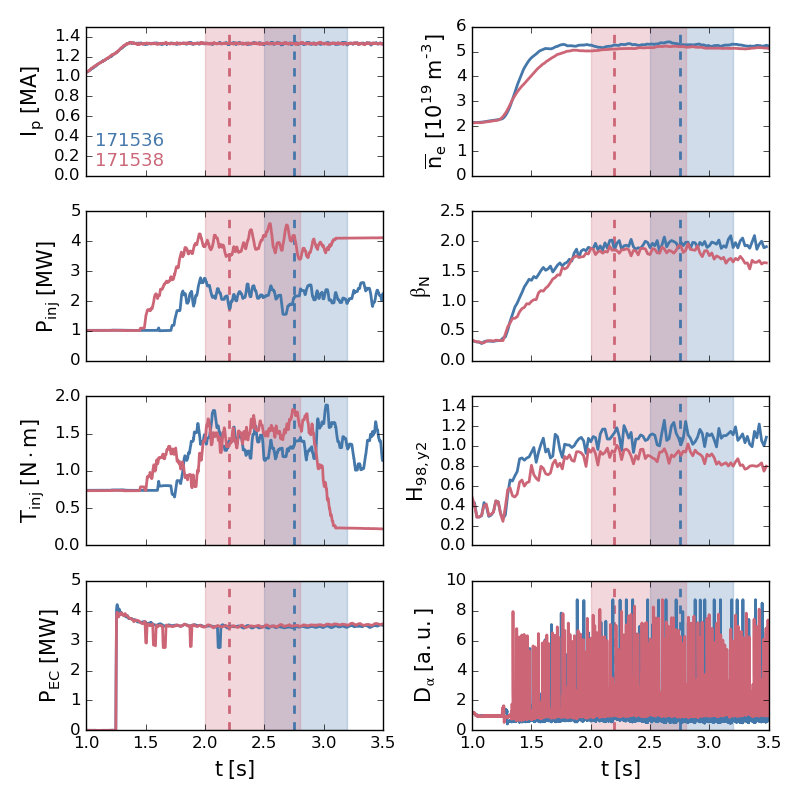
\includegraphics[width = \textwidth]{%
    Chapters/TurbulenceMeasurements/figs/traces.png}
  \caption[Time histories of various actuators \& plasma parameters]{%
    Time histories of various actuators and plasma parameters:
    (a) electron cyclotron resonance heating (ECH) power $P_{\text{ECH}}$,
    (b) ECH location $\rhoech$,
    (c) neutral beam injected (NBI) power $P_{\text{inj}}$,
    (d) NBI torque $T_{\text{inj}}$,
    (e) line-averaged density $\bar{n}_e$,
    (f) normalized plasma pressure $\beta_N$,
    (g) confinement quality $H_{98,\text{y}2}$, and
    (h) divertor $D_{\alpha}$ light, indicating
    the presence of large and small edge localized modes (ELMs).
  }
\label{fig:TurbulenceMeasurements:traces}
\end{figure}

\begin{figure}
  \centering
  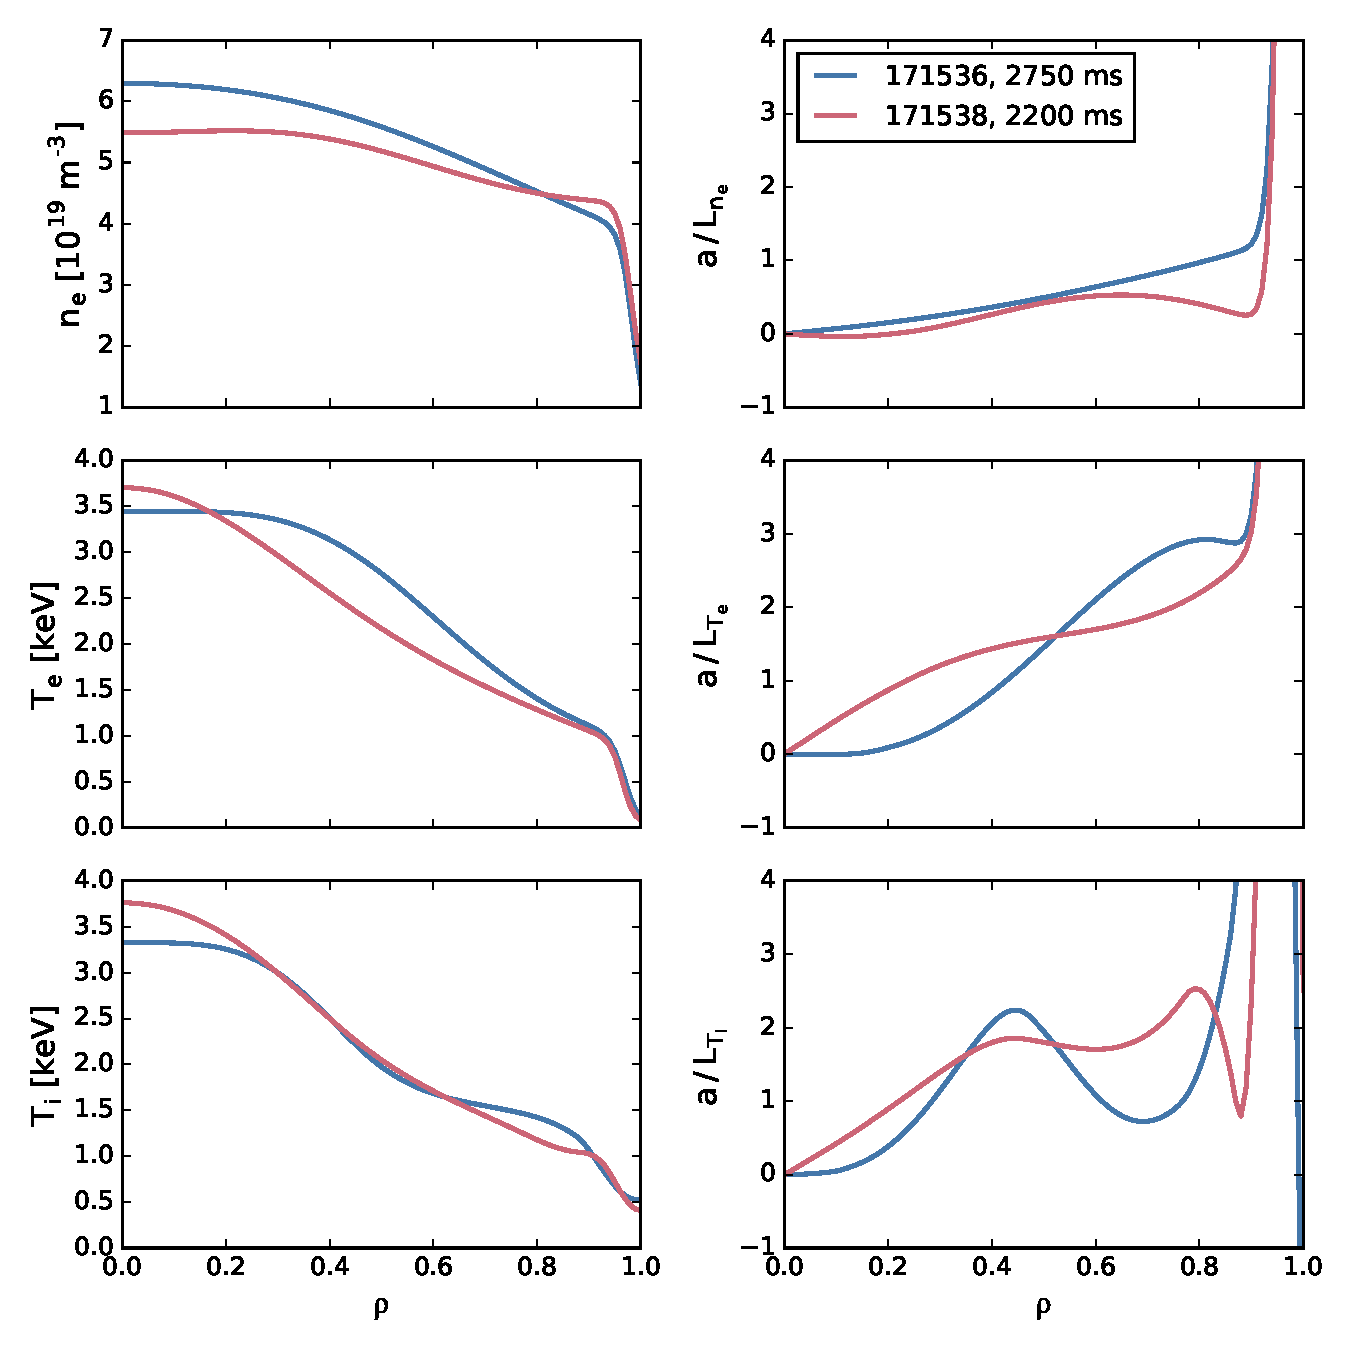
\includegraphics[width = \textwidth]{%
    Chapters/TurbulenceMeasurements/figs/profiles.pdf}
  \caption[Equilibrium profiles, inverse scale lengths, \& $\ExB$ shearing rate]{%
    Profiles, normalized inverse scale lengths, and $\ExB$ shearing rate:
    (a) electron density $n_e$,
    (b) electron temperature $T_e$,
    (c) deuterium temperature $T_i$,
    (d) radial electric field $E_r$ along the outboard midplane,
    (e) normalized inverse $n_e$ scale length $a / L_{n_e}$,
    (f) normalized inverse $T_e$ scale length $a / L_{T_e}$,
    (g) normalized inverse $T_i$ scale length $a / L_{T_i}$,
    (h) $\ExB$ shearing rate $\gamma_E$.
    The shaded bands indicate the $1\sigma$ uncertainties in the profiles,
    as determined by performing separate fits to $100$ distinct data sets
    generated via Monte Carlo variation
    of the measurements about their uncertainties.
    Representative measurements and their uncertainties are indicated
    for a $\SI{10}{\milli\second}$ window from a single shot.
    The relatively large uncertainty on $\gamma_E$
    is dominated by uncertainty in the curvature
    of the $T_i$ profile.
  }
\label{fig:TurbulenceMeasurements:profiles}
\end{figure}

Equilibrium profiles were obtained
by averaging over $\SI{200}{\milli\second}$,
as indicated by the shaded regions
in Figure~\ref{fig:TurbulenceMeasurements:traces}.
Magnetic equilibria were
reconstructed with the EFIT code~\cite{lao_fst05} and
were constrained to match the total plasma pressure and
motional Stark effect (MSE) measurements
of the local magnetic pitch angle.
Electron densities and temperatures
were measured via Thomson scattering, while
ion densities and temperatures
were inferred from charge exchange recombination (CER) measurements
of C$^{6+}$, the dominant impurity in \diiid.
The radial electric field was computed
by invoking force balance on C$^{6+}$.
% (poloidal data for $\rho \geq 0.6)$
To minimize the impact of ELMs on the profile fits,
only measurements falling
within the last {$50\%$ -- $99\%$} of each inter-ELM window
were included in the fitting.
The fitted profiles and
their corresponding gradients or
normalized inverse scale lengths
are shown in
Figure~\ref{fig:TurbulenceMeasurements:profiles}.
While it may seem counterintuitive
that the central electron temperature $T_e(0)$
increases when moving ECH from $\rho = 0.5$ to $\rho = 0.8$,
maintaining constant $\beta_N$
requires increased NBI heating
(see Figure~\ref{fig:TurbulenceMeasurements:traces}(c)),
which enhances the NBI electron heating density $q_{e,\text{NBI}}$
across the full plasma profile,
as shown in Figure~\ref{fig:TurbulenceMeasurements:electron_heating}(b).
The $1\sigma$ uncertainties in the profile fits,
indicated by the shaded bands in
Figure~\ref{fig:TurbulenceMeasurements:profiles},
were quantified by
performing separate fits to $100$ distinct data sets
generated via Monte Carlo variation
of the measurements about their uncertainties.
Clearly, moving ECH from $\rho = 0.5$ to $\rho = 0.8$
produces large changes
in the electron-scale and ion-scale drives,
$a / L_{T_e}$ and $a / L_{T_i}$, respectively,
in the region of the plasma accessible to the PCI probe beam
($R = \SI{1.98}{\meter}$).
Using these profiles,
power-balance analysis was performed
with the ONETWO code~\cite{pfeiffer_onetwo},
with NUBEAM~\cite{pankin_cpc04} calculations
for NBI heating and torque and
TORAY~\cite{matsuda_ieee89} calculations for ECH;
the resulting loop voltages, stored energies, and neutron rates
match their measured values to within $\pm 5\%$.

\begin{figure}
  \centering
  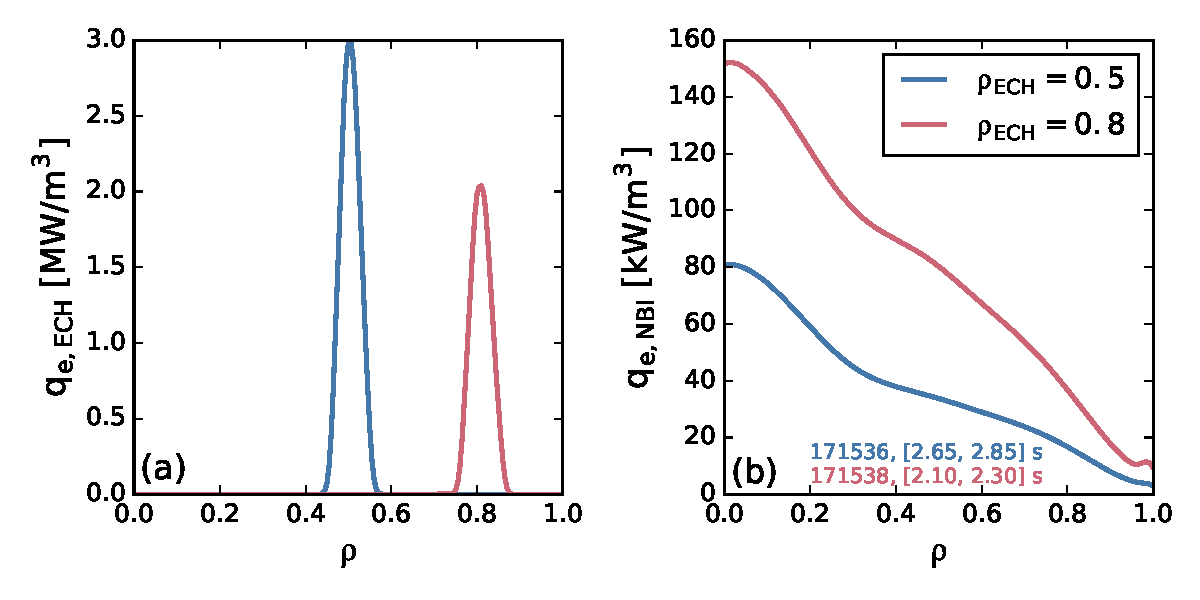
\includegraphics[width = \textwidth]{%
    Chapters/TurbulenceMeasurements/figs/electron_heating.pdf}
  \caption[ECH \& NBI electron-heating profiles]{%
    (a) ECH electron heating density $q_{e,\text{ECH}}$ and
    (b) NBI electron heating density $q_{e,\text{NBI}}$.
    When moving ECH from $\rho = 0.5$ to $\rho = 0.8$,
    maintaining constant $\beta_N$
    requires increased NBI heating
    (see Figure~\ref{fig:TurbulenceMeasurements:traces}(c)),
    which enhances the NBI electron heating density $q_{e,\text{NBI}}$
    across the full plasma profile.
    The radiated power and ohmic heating
    negligibly change between the two discharges.
  }
\label{fig:TurbulenceMeasurements:electron_heating}
\end{figure}


\section{Combined PCI-interferometer measurements}
\label{sec:TurbulenceMeasurements:Measurements}
The experiment described in
Section~\ref{sec:TurbulenceMeasurements:ExperimentalConditions}
presents an ideal opportunity
for multiscale turbulence investigations
with the combined PCI-interferometer.
Below, Section~\ref{sec:TurbulenceMeasurements:Measurements:ELM_filtering}
discusses the automated filtering of transient bursts
attributable to edge localized modes (ELMs)
that would otherwise bias spectral estimates
of the background turbulence.
Section~\ref{sec:TurbulenceMeasurements:Measurements:Sf} then
compares the interferometer and PCI frequency spectra
for $\rhoech = 0.5$ and $\rhoech = 0.8$;
interestingly, the interferometer identifies
a novel turbulent branch with properties
consistent with a micro-tearing mode (MTM).
Next, Section~\ref{sec:TurbulenceMeasurements:Measurements:Skf}
presents the PCI frequency-wavenumber spectra,
which reveal the presence of several distinct turbulent branches.
Finally, Section~\ref{sec:TurbulenceMeasurements:Measurements:Sk}
demonstrates that the PCI wavenumber spectrum
distinctly flattens with $\rhoech = 0.5$
relative to that with $\rhoech = 0.8$,
which is reminiscent of results
from realistic multiscale gyrokinetic simulations.


\subsection{ELM filtering}
\label{sec:TurbulenceMeasurements:Measurements:ELM_filtering}
Edge localized modes (ELMs) expel impurities from the plasma but
will also present severe challenges to plasma-facing components
in future reactors~\cite[Sec.~7.17]{wesson}.
Because of their virulence and their bursty nature,
ELMs produce strong spiking in the interferometer and PCI measurements,
whitening the measured spectra
[Sec.~10.3.2.3]\cite{bendat_and_piersol}.
Additionally, the temperature and density profiles relax during an ELM,
altering the turbulent drives in the plasma edge.
In order to accurately estimate
the spectrum of the background turbulence, then,
the ELM contributions to the interferometer and PCI measurements
must be removed.

\begin{figure}
  \centering
  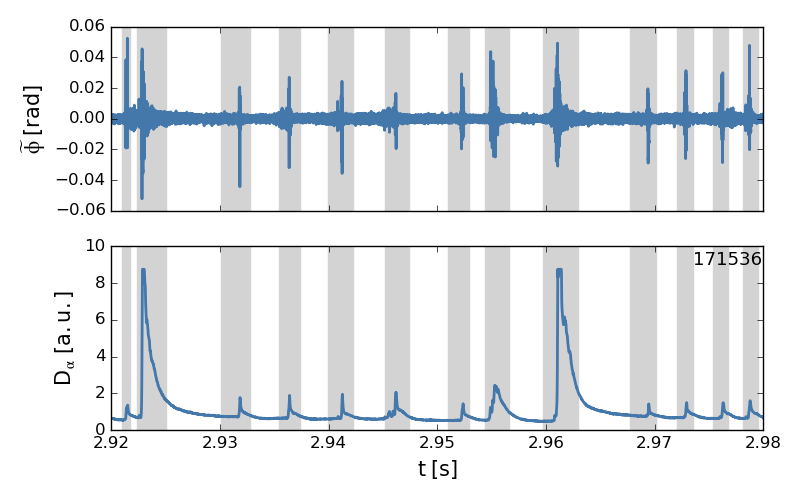
\includegraphics[width = \textwidth]{%
    Chapters/TurbulenceMeasurements/figs/ELM_filtering_example.png}
  \caption[ELM filtering]{%
    Edge localized modes (ELMs) must be removed
    from the PCI and interferometer measurements
    prior to spectral analysis of the background turbulence.
    (Upper panel): The interferometer-measured
    fluctuating phase $\tilde{\phi}$,
    with large, ELM-induced spiking.
    (Lower panel): Divertor $D_{\alpha}$ emission,
    indicating the presence of large Type I ELMs
    as well as smaller ELMs.
    Windows \emph{excluded} from spectral analysis are shown in gray.
    The \diiid\space shot number is shown in the upper right
    of the lower panel.
  }
\label{fig:TurbulenceMeasurements:ELM_filtering_example}
\end{figure}

In this work, ELMs are simply and automatically detected
using measurements from the interferometer.
After the high-pass filtering described in
Section~\ref{sec:Implementation:DataPreparation:high_pass_filtering},
the interferometer-measured fluctuating phase $\tilde{\phi}$
is a zero-mean, random process,
as shown in the upper panel of
Figure~\ref{fig:TurbulenceMeasurements:ELM_filtering_example}.
Large, intermittent spikes pepper $\tilde{\phi}(t)$ during ELMy H-mode, and
the lower panel of
Figure~\ref{fig:TurbulenceMeasurements:ELM_filtering_example}
indicates that these spikes are well correlated
with ELM-induced $D_{\alpha}$ emission in the divertor.
While the $D_{\alpha}$ emission following large Type I ELMs
exhibits a relatively slow decay,
the interferometer-measured $\tilde{\phi}$
returns to stationarity much more rapidly.
Thus, it is desirable to identify
stationary inter-ELM windows
from the interferometer measurements
rather than the $D_{\alpha}$ emission.
Points in the interferometer-measured $\tilde{\phi}$
exceeding $3 \times$ the RMS value
are identified as ELMs, and
successive ELMs are required to be separated
by at least a $\SI{0.5}{\milli\second}$ ``debouncing time''
(spikes separated by less than the debouncing time
are classified as belonging to the same ELM).
Subsequent spectral analysis is then performed
using only the $20\%$ -- $80\%$ inter-ELM windows
of the interferometer and PCI measurements.
Figure~\ref{fig:TurbulenceMeasurements:ELM_filtering_example}
shows the windows \emph{excluded} from spectral analysis in gray.


\subsection{Frequency spectra}
\label{sec:TurbulenceMeasurements:Measurements:Sf}
One-sided autospectral densities estimates $G_{\phi,\phi}(f)$
of the phase fluctuations
are calculated using the methodology
described in Section~\ref{app:SpectralEstimation:NonParametric}.
The interferometer and PCI signals
from the shaded windows in
Figure~\ref{fig:TurbulenceMeasurements:traces}
are split into realizations of $1024$ points
(corresponding to roughly $\SI{250}{\micro\second}$)
resulting in a frequency resolution
of approximately $\SI{4}{\kilo\hertz}$ in the spectral estimates.
As described in
Section~\ref{sec:TurbulenceMeasurements:Measurements:ELM_filtering},
only realizations falling within
$20\%$ -- $80\%$ of each inter-ELM window
are included in the ensemble averaging;
the exact number of realizations $N_r$
included in each ensemble
depends on the details of the ELM dynamics, but
$N_r \sim 450$ for the shots considered here,
corresponding to a relative random error
in $G_{\phi,\phi}(f)$ of approximately $5\%$.
A Hanning window is applied to each realization
prior to computation of its fast Fourier transform (FFT).
To simplify inter-ELM bookkeeping,
adjacent realizations have zero overlap.
As described in
Section~\ref{sec:Implementation:DataPreparation:high_pass_filtering},
the interferometer and PCI phase signals
are high-pass filtered prior to spectral analysis, and
no further detrending is performed.
The resulting spectral estimates
for $\rhoech = 0.5$ and $\rhoech = 0.8$
are shown in
Figure~\ref{fig:TurbulenceMeasurements:Sf_interferometer_pci}.
The corresponding noise floors are estimated
from $\SI{50}{\milli\second}$ of data
prior to plasma breakdown;
the knee in the PCI noise floor
at approximately $\SI{500}{\kilo\hertz}$
corresponds to the roll-off in the temporal bandwidth
of the PCI detector and its preamplifiers.
As expected theoretically
(see Figure~\ref{fig:InterferometricMethods:interferometric_method_transfer_functions})
and observed empirically in sound-wave calibrations
(see Figure~\ref{fig:Implementation:cross_calibration}),
the PCI is more sensitive than the heterodyne interferometer.

\begin{figure}
  \centering
  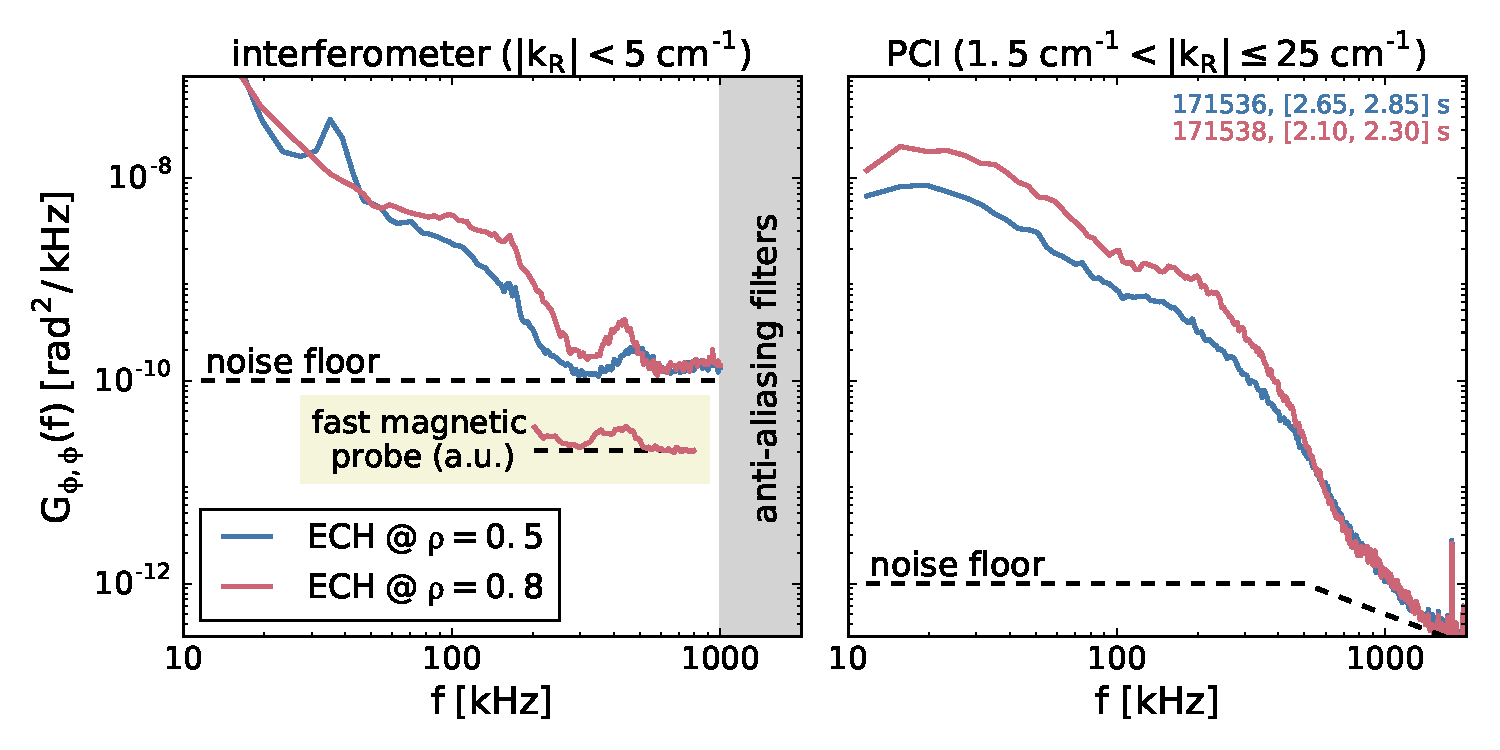
\includegraphics[width = \textwidth]{%
    Chapters/TurbulenceMeasurements/figs/Sf_interferometer_pci.pdf}
  \caption[Interferometer \& PCI frequency spectra]{%
    One-sided autospectral-density estimates $G_{\phi,\phi}(f)$ from
    (a) the heterodyne interferometer and (b) the PCI.
    The low-frequency ($f \lesssim \SI{300}{\kilo\hertz}$) dynamics
    are comparable, with both the interferometer and the PCI
    measuring a $2 - 4\times$ increase in fluctuation power
    when moving from $\rhoech = 0.5$ to $\rhoech = 0.8$.
    The higher-frequency ($f \gtrsim \SI{300}{\kilo\hertz}$) dynamics,
    however, are distinct.
    In particular, the interferometer-measured broadband fluctuation
    between $\SI{300}{\kilo\hertz}$ and $\SI{600}{\kilo\hertz}$
    is low-$k$ (due to its absence in the PCI spectrum),
    electromagnetic (as seen by the beige inset to (a)), and
    driven by collisionality
    (as shown in Figure~\ref{fig:TurbulenceMeasurements:collisionality}),
    suggesting that it may be a micro-tearing mode (MTM).
    The subtle break in slope at $f \sim \SI{800}{\kilo\hertz}$
    in the PCI spectrum when $\rhoech = 0.8$
    is shown to be a distinct turbulent branch
    in Figure~\ref{fig:TurbulenceMeasurements:Skf_pci}.
  }
\label{fig:TurbulenceMeasurements:Sf_interferometer_pci}
\end{figure}

Interestingly, the autospectral density of the heterodyne interferometer
indicates the presence of a distinct broadband fluctuation
with a central frequency $f_0 \sim \SI{450}{\kilo\hertz}$ and
a bandwidth $\Delta f \sim \SI{300}{\kilo\hertz}$.
The toroidally separated $V2$ interferometer
corroborates the presence of this fluctuation, but
the fluctuation is only vaguely coherent between the two interferometers,
with magnitude-squared coherences $\gamma_{xy}^2(f) \leq 0.1$.
The fluctuation is larger than
the corresponding PCI-measured fluctuations
in this frequency range, but
it is absent from the autospectral density of the PCI;
this indicates that the fluctuation wavenumber
is smaller than the PCI low-$k$ cutoff
(\ref{eq:Implementation:kg_realized}).
Further, this fluctuation has a magnetic component,
as shown by the beige inset to
Figure~\ref{fig:TurbulenceMeasurements:Sf_interferometer_pci}(a).
The red curve in the beige inset
corresponds to the autospectral density (in arbitrary units)
of the poloidal magnetic-field fluctuations
measured by a high-frequency magnetic probe ($b5$)~\cite{strait_rsi06}
during the $\rhoech = 0.8$ window, while
the dashed line corresponds to the noise floor,
as estimated from $\SI{50}{\milli\second}$
of data prior to plasma breakdown.
The magnetic autospectral density is estimated
in a manner consistent with those of the interferometer and PCI
(realization length of approximately $\SI{250}{\micro\second}$
with zero overlap between adjacent realizations,
application of Hanning window to each realization prior to FFT computation,
ensemble averaging only over realizations falling within
$20\%$ -- $80\%$ of each inter-ELM window, and
a total number of realizations $N_r \sim 450$).
The autospectral density of the interferometer also
indicates that the power in this fluctuation
increases when moving from
$\rhoech = 0.5$ to $\rhoech = 0.8$.
To prove that this is a robust trend,
the total power in this fluctuation
is computed for stationary windows
from $7$ distinct shots with $\rhoech = 0.5$ and
from $7$ distinct shots with $\rhoech = 0.8$,
each of which are nominally identical
to the corresponding discharges shown in
Figures~\ref{fig:TurbulenceMeasurements:traces} and
\ref{fig:TurbulenceMeasurements:profiles}.
The total fluctuation power is quantified as
\begin{equation}
  \text{var}(\tilde{\phi})
  =
  \int_{\SI{300}{\kilo\hertz}}^{\SI{600}{\kilo\hertz}}
  \left[%
    G_{\phi,\phi}^{\text{int}}(f) - N.F.
  \right] df,
  \label{eq:TurbulenceMeasurements:MTM_power}
\end{equation}
where $G_{\phi,\phi}^{\text{int}}(f)$
is the autospectral density of the heterodyne interferometer and
$N.F. = \SI{e-10}{\radian\squared\per\kilo\hertz}$
is the corresponding noise floor.
\begin{figure}
  \centering
  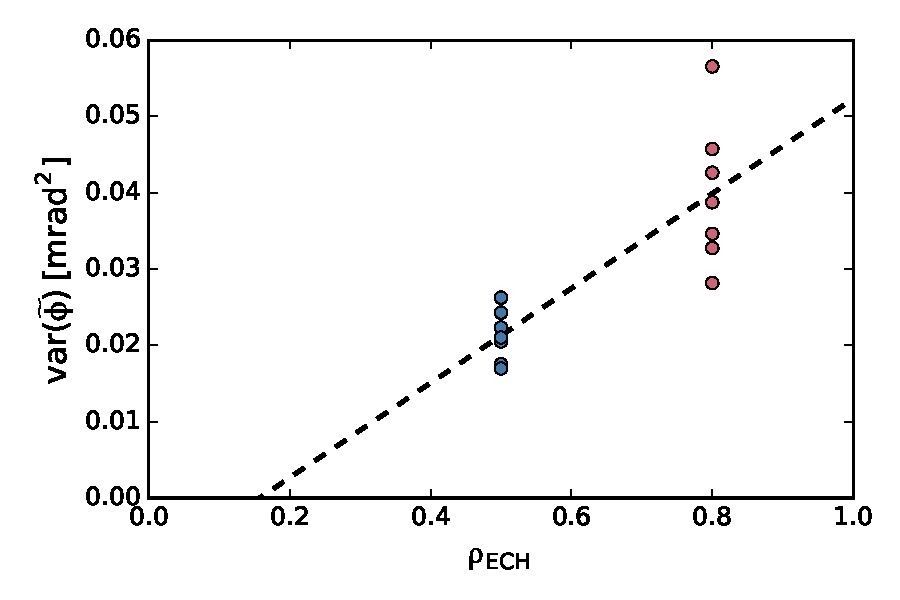
\includegraphics[width = 0.75 \textwidth]{%
    Chapters/TurbulenceMeasurements/figs/interferometer_bump_integrated_power.pdf}
  \caption[Power in low-$k$, mid-$f$, electromagnetic turbulence vs. ECH location]{%
    Power $\text{var}(\tilde{\phi})$ in interferometer-measured
    low-$k$, mid-$f$, electromagnetic turbulence vs. ECH location $\rhoech$.
    Powers are estimated via
    (\ref{eq:TurbulenceMeasurements:MTM_power}).
    Different points correspond to distinct, nominally identical shots
    from the same experimental run day;
    the dashed line is the linear least-squares fit to the points,
    indicating an approximate doubling in fluctuation power
    when moving from $\rhoech = 0.5$ to $\rhoech = 0.8$.
  }
\label{fig:TurbulenceMeasurements:interferometer_bump_integrated_power}
\end{figure}
Figure~\ref{fig:TurbulenceMeasurements:interferometer_bump_integrated_power}
plots $\text{var}(\tilde{\phi})$ versus $\rhoech$;
a linear least-squares fit
indicates that the fluctuation power
approximately doubles when moving
from $\rhoech = 0.5$ to $\rhoech = 0.8$.
Further, Figure~\ref{fig:TurbulenceMeasurements:collisionality}
shows that the electron-ion collisionality $\nu_{ei}$
in the region of the plasma accessible to the PCI probe beam
($R = \SI{1.98}{\meter}$)
also roughly doubles when moving
from $\rhoech = 0.5$ to $\rhoech = 0.8$.
Thus, this fluctuation is
low-$k$, electromagnetic, and driven by collisionality,
suggesting that this fluctuation
may be a micro-tearing mode (MTM)~\cite[Sec.~8.5]{wesson}\cite{drake_pf77},
which is predicted to be marginally unstable
in this experiment's reference discharge~\cite{holland_nf17}.

\begin{figure}
  \centering
  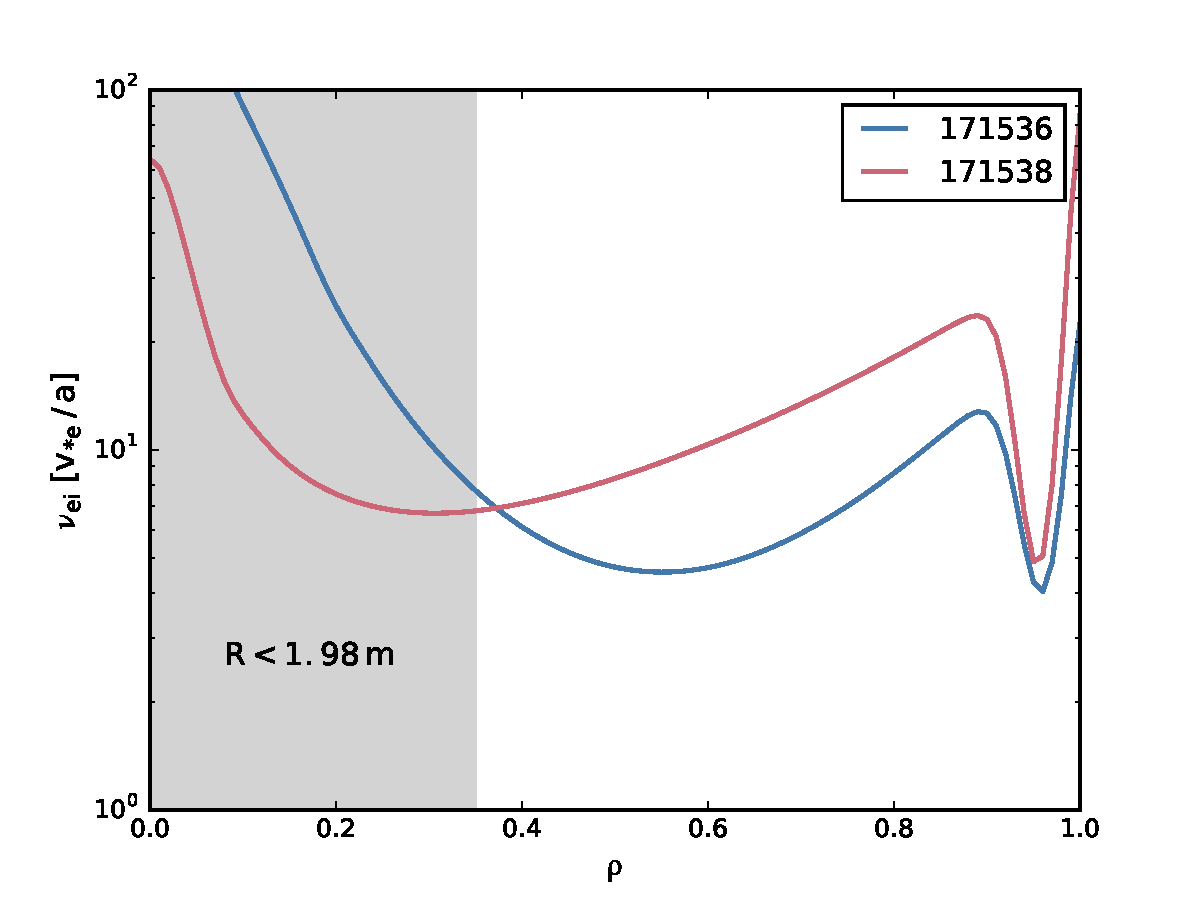
\includegraphics[width = 0.9 \textwidth]{%
    Chapters/TurbulenceMeasurements/figs/collisionality.pdf}
  \caption[Collisionality variation with ECH location]{%
    The electron-ion collisionality $\nu_{ei}$
    in the region of the plasma
    accessible to the PCI probe beam
    ($R = \SI{1.98}{\meter}$)
    roughly doubles when moving
    from $\rhoech = 0.5$ to $\rhoech = 0.8$.
    The collisionality is computed from the profiles in
    Figure~\ref{fig:TurbulenceMeasurements:profiles}, and
    the shaded bands indicate the $1\sigma$ uncertainties.
    The collisionality normalization is $\vmag_{*e} / a$, where
    $\vmag_{*e}$ is the electron diamagnetic velocity and
    $a$ is the minor radius of the plasma;
    note that the angular electron diamagnetic frequency
    $\omega_{*e} \propto \vmag_{*e} / a$~\cite[Sec.~8.2]{wesson} and
    that micro-tearing mode (MTM) linear-stability calculations
    are performed in expansions of $\nu_{ei} / \omega_{*e}$
    \cite[Sec.~8.5]{wesson}\cite{drake_pf77}.
    Unfortunately, without a wavenumber measurement,
    the more theoretically relevant $\omega_{*e}$ normalization
    cannot be performed.
    Both discharges are in the banana regime
    ($\nu_{ei}^* < 1$)~\cite[Sec.~4.6]{wesson}
    for $\rho \lesssim 0.95$.
  }
\label{fig:TurbulenceMeasurements:collisionality}
\end{figure}

It is also interesting to examine
the low-frequency ($f \lesssim \SI{300}{\kilo\hertz}$) fluctuations
measured by both the interferometer and the PCI.
Both systems measure a $2 - 4\times$ increase
in the low-frequency fluctuation power
when moving from $\rhoech = 0.5$ to $\rhoech = 0.8$,
which may be responsible for the slightly reduced confinement
in Figure~\ref{fig:TurbulenceMeasurements:traces}(g).
The spatial content of these fluctuations
can be roughly characterized
via the magnitude-squared coherence $\gamma^2_{xy}(f)$
between the interferometer ($x$) and PCI ($y$) measurements.
As discussed in Section~\ref{app:SpectralEstimation:NonParametric},
$\gamma^2_{xy}(f)$ is bounded between $0$ and $1$, and
it quantifies the linear correlation between signals $x$ and $y$,
with $\gamma^2_{xy}(f) = 0$ indicating $0\%$ correlation at frequency $f$ and
$\gamma^2_{xy}(f) = 1$ indicating $100\%$ correlation at frequency $f$.
Thus, $\gamma^2_{xy}(f)$ characterizes the fraction of fluctuation power
sitting in the mid-$k$ overlap of the interferometer and PCI
\cite[Sec.~5.2.6]{bendat_and_piersol}.
As with the auto-spectral density estimates,
the interferometer and PCI signals
are split into realizations of $1024$ points
with zero overlap between adjacent realizations,
a Hanning window is applied to each realization
prior to computing its FFT,
the ensemble average is performed only over realizations falling within
$20\%$ -- $80\%$ of each inter-ELM window, and
the total number of realizations is $N_r \sim 450$.
The resulting $\gamma^2_{xy}(f)$ estimates
are shown in Figure~\ref{fig:TurbulenceMeasurements:gamma2xy}.
As demonstrated in Section~\ref{sec:TurbulenceMeasurements:Measurements:Skf},
the frequency $f$ of a broadband fluctuation
is often related to its wavenumber $k$ via
$f = \vph k / (2 \pi)$,
where $\vph$ is the lab-frame phase velocity of the fluctuation;
that is, the lowest frequencies in a particular fluctuation branch
are associated with the lowest wavenumbers, and
the highest frequencies in a particular fluctuation branch
are associated with the highest wavenumbers.
Thus, the low values of $\gamma^2_{xy}(f)$
for $f \lesssim \SI{100}{\kilo\hertz}$
in Figure~\ref{fig:TurbulenceMeasurements:gamma2xy}
can be interpreted as the interferometer measuring
substantial power in low-$k$ fluctuations
that sit below the PCI's low-$k$ cutoff
(\ref{eq:Implementation:kg_realized}).
Similarly, the low values of $\gamma^2_{xy}(f)$
for $f \gtrsim \SI{300}{\kilo\hertz}$
correspond to the PCI measuring
substantial power in high-$k$ fluctuations
that sit above the interferometer's high-$k$ cutoff
(\ref{eq:Implementation:kfsv_interferometer_design})
or below the interferometer's noise floor.
Between $\SI{100}{\kilo\hertz}$ and $\SI{300}{\kilo\hertz}$,
$0.25 \lesssim \gamma^2_{xy} \lesssim 0.5$,
indicating between $25\%$ and $50\%$
of the total fluctuation power
sits in the mid-$k$ overlap of the interferometer and the PCI.
Further, moving from $\rhoech = 0.5$ to $\rhoech = 0.8$
produces a substantial increase in $\gamma^2_{xy}(f)$
for $\SI{200}{\kilo\hertz} \lesssim f \lesssim \SI{300}{\kilo\hertz}$,
suggesting that the wavenumbers of these fluctuations decrease
when moving from $\rhoech = 0.5$ to $\rhoech = 0.8$;
this is corroborated by the increase in the lab-frame phase velocity
shown in Figure~\ref{fig:TurbulenceMeasurements:Skf_pci}.

\begin{figure}
  \centering
  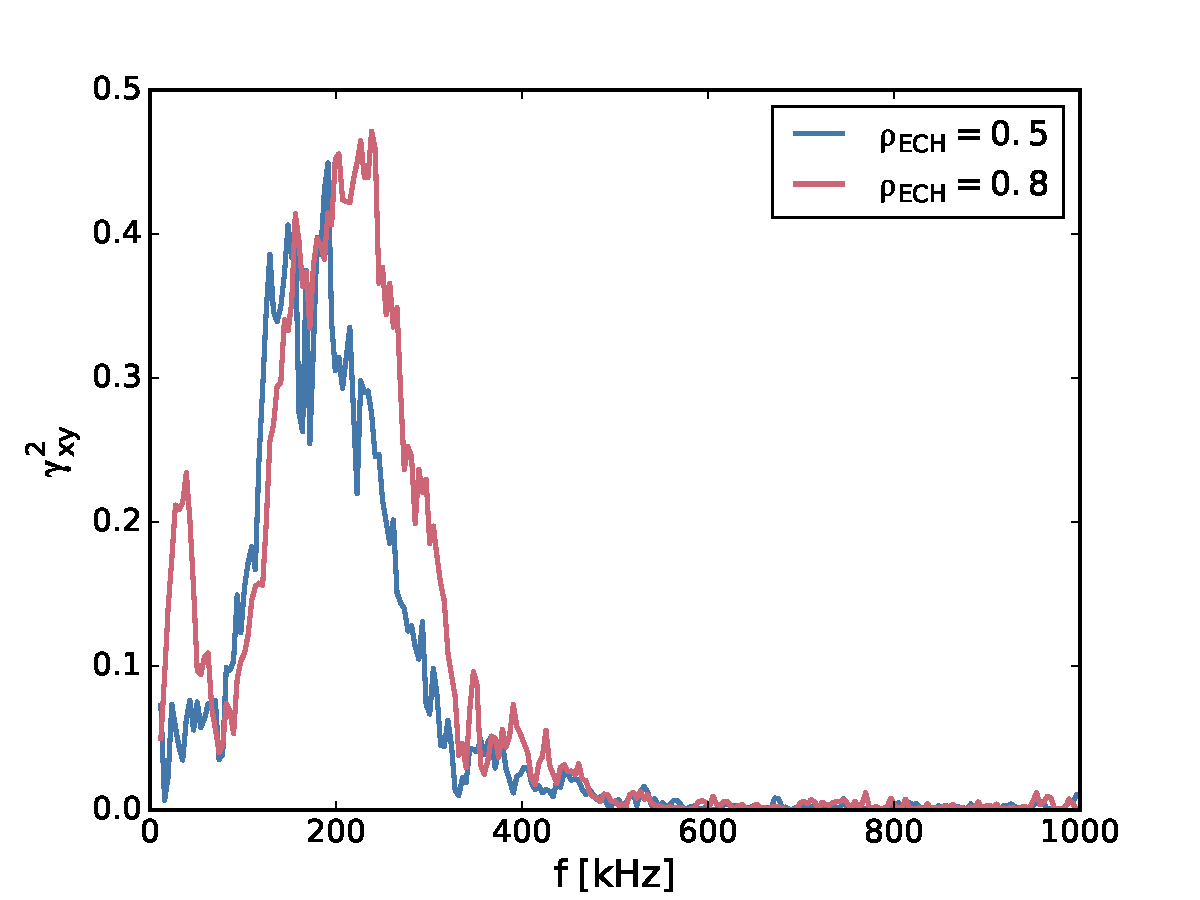
\includegraphics[width = 0.85 \textwidth]{%
    Chapters/TurbulenceMeasurements/figs/coherence.pdf}
  \caption[Magnitude-squared coherence between interferometer \& PCI]{%
    The magnitude-squared coherence $\gamma^2_{xy}(f)$
    between the interferometer and the PCI measurements
    characterizes the fraction of total fluctuation power
    sitting in the mid-$k$ overlap of the interferometer and the PCI.
    The increase in $\gamma^2_{xy}(f)$
    between $\SI{200}{\kilo\hertz}$ and $\SI{300}{\kilo\hertz}$
    when moving from
    $\rhoech = 0.5$ to $\rhoech = 0.8$
    suggests a wavenumber downshift in these fluctuations, which
    is corroborated by the increase in the lab-frame phase velocity
    shown in Figure~\ref{fig:TurbulenceMeasurements:Skf_pci}.
  }
  \label{fig:TurbulenceMeasurements:gamma2xy}
\end{figure}


\subsection{Frequency-wavenumber spectra}
\label{sec:TurbulenceMeasurements:Measurements:Skf}
As the PCI measurements are made
with a multi-element detector array,
the spatial content of the PCI signal
can also be characterized.
The two-dimensional autospectral density $S_{\phi,\phi}(k,f)$
simultaneously quantifies the spatial and temporal content of a signal.
(Unfortunately, as the interferometer measurements
are currently made with a single-element detector,
$S_{\phi,\phi}(k, f)$ cannot be estimated
from the interferometer measurements;
the only spatial knowledge about the interferometer signal
is that the wavenumber magnitudes $|k|$
sit below the interferometer's high-$k$ cutoff
(\ref{eq:Implementation:kfsv_interferometer_design})).

The PCI $S_{\phi,\phi}(k, f)$ is estimated using the hybrid
non-parametric-in-time, parametric-in-space technique
discussed in Section~\ref{app:SpectralEstimation:2d_spectra:2d_spectra}.
Specifically, the hybrid autocorrelation function
$\tilde{R}_{\phi,\phi}(\delta, f)$ is estimated non-parametrically
over the shaded windows in Figure~\ref{fig:TurbulenceMeasurements:traces}
via (\ref{eq:SpectralEstimation:hybrid_autocorrelation_estimate})
using the same spectral-estimation parameters as those
in Section~\ref{sec:TurbulenceMeasurements:Measurements:Sf}
(i.e.\ realization length of $1024$ points with
zero overlap between adjacent realizations,
application of Hanning window to each realization prior to FFT computation,
ensemble averaging only over realizations falling within
$20\%$ -- $80\%$ of each inter-ELM window, and
a total number of realizations $N_r \sim 450$).
Then, a parametric $p = 6$ Burg autoregression (AR)
in the spatial lag $\delta$
estimates the autospectral density $S_{\tilde{R},\tilde{R}}(k,f)$
of $\tilde{R}(\delta, f)$, and
the autospectral density $S_{\phi,\phi}(k, f)$
of the phase fluctuations is computed
via (\ref{eq:SpectralEstimation:autospectral_density_Burg}).
The Burg AR is evaluated
on a uniformly spaced, $1000$-element wavenumber grid.
Often, an AR model is referred to as an ``all-pole model''
because the only frequency dependence in the spectral estimate
appears in the denominator;
this all-pole feature of an AR model
allows fitting very sharp spectral features and
substantially improves the wavenumber resolution
of the sparsely sampled (in space) PCI data
(see Figure~\ref{fig:SpectralEstimation:Skf_example}
for a comparison to a conventional Fourier-in-space estimate).

\begin{figure}
  \centering
  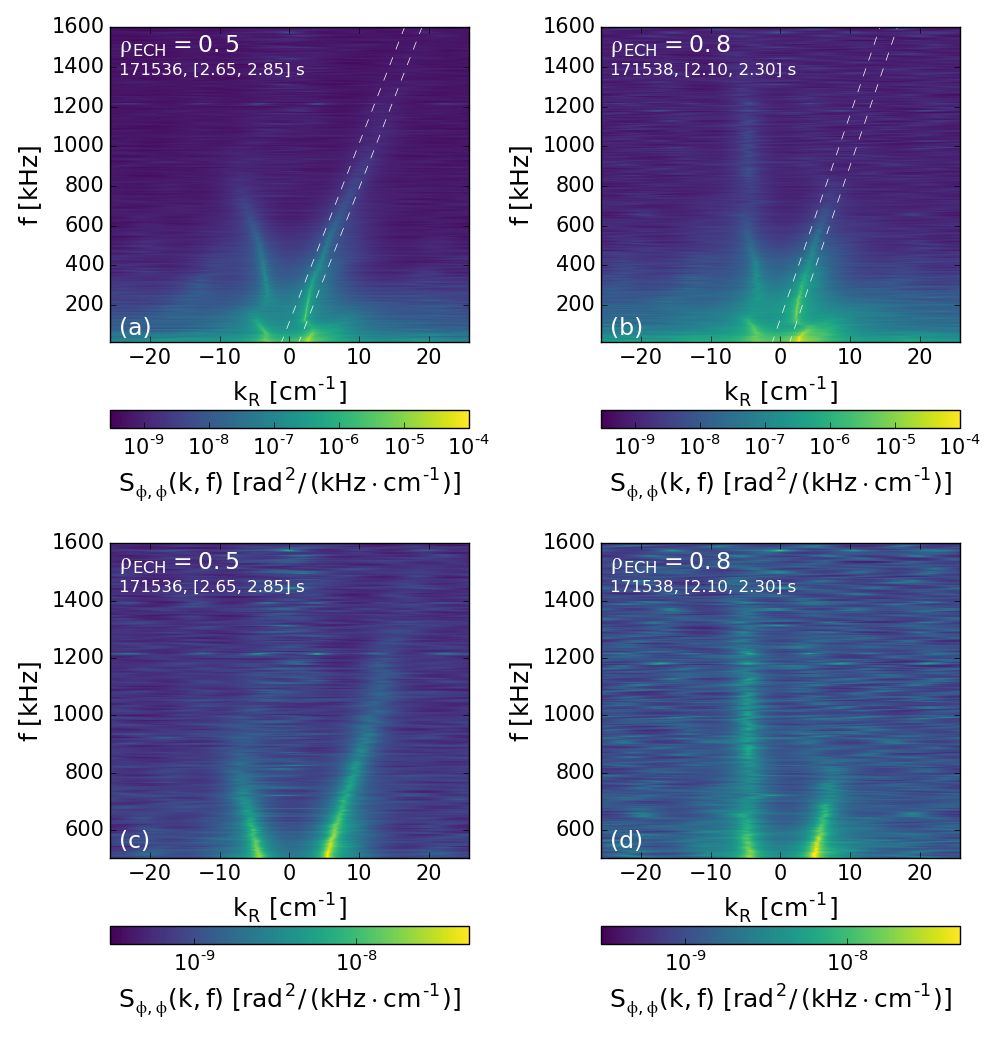
\includegraphics[width = \textwidth]{%
    Chapters/TurbulenceMeasurements/figs/Skf_pci_zoom.png}
  \caption[PCI frequency-wavenumber spectra]{%
    PCI two-dimensional autospectral densities $S_{\phi,\phi}(k, f)$
    for (a) $\rhoech = 0.5$ and (b) $\rhoech = 0.8$.
    To better resolve the high-$k$ and high-$f$ features,
    (c) and (d) display the same spectra from (a) and (b), respectively,
    but only for $f \geq \SI{500}{\kilo\hertz}$ and
    with an altered colorscale.
    Moving from $\rhoech = 0.5$ to $\rhoech = 0.8$
    increases the lab-frame phase velocity but
    decreases the spatiotemporal bandwidth
    of the broadband turbulence bounded by
    the annotating dashed white lines and
    also excites a new turbulent branch
    at $k \sim \SI{-5}{\per\centi\meter}$ and
    $f \sim \SI{1}{\mega\hertz}$.
  }
\label{fig:TurbulenceMeasurements:Skf_pci}
\end{figure}

The PCI $S_{\phi,\phi}(k, f)$
for $\rhoech = 0.5$ and $\rhoech = 0.8$ are shown in
Figure~\ref{fig:TurbulenceMeasurements:Skf_pci}.
The spectra indicate the existence of numerous turbulent branches,
each of which may respond differently when $\rhoech$ is varied.
Two of these branches are discussed here.
First, perhaps one of the most surprising qualitative effects
of moving $\rhoech = 0.5$ to $\rhoech = 0.8$
is the excitation of a new, distinct turbulent mode
at $k_R \sim \SI{-5}{\per\centi\meter}$
with a central frequency $f_0 \sim \SI{1}{\mega\hertz}$ and
a bandwidth $\Delta f \sim \SI{400}{\kilo\hertz}$.
This mode corresponds to the subtle break in slope
at $f \sim \SI{800}{\kilo\hertz}$ in the PCI $G_{\phi,\phi}(f)$
in Figure~\ref{fig:TurbulenceMeasurements:Skf_pci}.
This mode straddles
the current spatiotemporal limits of the interferometer and
sits well below the interferometer noise floor;
thus, this mode is invisible to the interferometer.
The mode is robustly observed in all $7$
of the steady-state $\rhoech = 0.8$ windows
from this experimental run day, and
it is robustly absent from all $7$
of the corresponding $\rhoech = 0.5$ windows.
It should be noted that
the PCI observes a similar mode
during ELM-free H-mode and
wide-pedestal QH-mode~\cite{rost_med_k_high_f_mode}
as well as during NBI-only ELMy H-mode
(see Figure~\ref{fig:SpectralEstimation:Skf_example}).
Second, and perhaps of more relevance to multiscale studies,
is the turbulent branch
bounded by the annotating dashed white lines
in Figure~\ref{fig:TurbulenceMeasurements:Skf_pci}.
When $\rhoech = 0.5$,
this turbulent branch
has a lab-frame phase velocity
$\vph = \SI{5.6}{\kilo\meter\per\second}$
with wavenumbers and frequencies extending to
$\SI{14}{\per\centi\meter}$ and $\SI{1250}{\kilo\hertz}$, respectively;
moving to $\rhoech = 0.8$
increases the lab-frame phase velocity to
$\vph = \SI{6.5}{\kilo\meter\per\second}$
but reduces the spatiotemporal bandwidth to
$\SI{7.2}{\per\centi\meter}$ and $\SI{750}{\kilo\hertz}$.
These observations are generic to all $7$
of the steady-state $\rhoech = 0.5$ windows
and all $7$ of the steady-state $\rhoech = 0.8$ windows
from this experimental run day.
Note that for a given frequency $f$,
an increase in phase velocity
corresponds to a wavenumber downshift
such that the observed change in $\vph$ with $\rhoech$
confirms the wavenumber-downshift speculation
from Figure~\ref{fig:TurbulenceMeasurements:gamma2xy}.
This turbulent branch will be investigated further
in Section~\ref{sec:TurbulenceMeasurements:Measurements:Sk}.


\subsection{Wavenumber spectra}
\label{sec:TurbulenceMeasurements:Measurements:Sk}
Because simulations are finely sampled in space
but often have limited temporal histories,
experimental wavenumber spectra
are particularly valuable for validating
theoretical models and computational predictions.
The PCI wavenumber autospectral density $S_{\phi,\phi}(k)$
corresponding to a given turbulent branch
is computed by integrating the
two-dimensional autospectral density $S_{\phi,\phi}(k, f)$
from Section~\ref{sec:TurbulenceMeasurements:Measurements:Skf}
over the temporal bandwidth $\Delta f$ of the turbulent branch, i.e.\
\begin{equation}
  S_{\phi,\phi}(k)
  =
  \int_{f_0(k) - (\Delta f / 2)}^{f_0(k) + (\Delta f / 2)}
  S_{\phi,\phi}(k, f) df,
\end{equation}
where $f_0(k) = k \vph / (2 \pi)$
is the central frequency of the turbulent branch at wavenumber $k$, and
$\vph$ is the lab-frame phase velocity of the turbulent branch.
Note that restricting the integration domain in this manner
minimizes contributions to $S_{\phi,\phi}(k)$
from noise outside of the branch's bandwidth.
For example, integrating between the bounds
denoted by the annotating dashed white lines
in Figure~\ref{fig:TurbulenceMeasurements:Skf_pci}
produces the $S_{\phi,\phi}(k)$ displayed
in Figure~\ref{fig:TurbulenceMeasurements:Sk_power_law}.
Note that the $\rhoech = 0.5$ spectrum
is substantially flattened (i.e.\ decays more slowly)
relative to the $\rhoech = 0.8$ spectrum.
As shown in Figure~\ref{fig:TurbulenceMeasurements:profiles},
relative to $\rhoech = 0.8$,
$\rhoech = 0.5$ corresponds to
increased $a / L_{Te}$ and decreased $a / L_{T_i}$
over the majority of the plasma
accessible to the PCI probe beam
($R = \SI{1.98}{\meter}$).
This spectral flattening with
enhanced electron-scale drive relative to ion-scale drive
is reminiscent of results from
multiscale gyrokinetic simulations~\cite{howard_pp16}
of an ion cyclotron resonance heated (ICRH)~\cite[Sec.~5.8]{wesson}
L-mode discharge in Alcator C-Mod~\cite[Sec.~11.5]{wesson}.
While the only existing, realistic, multiscale gyrokinetic simulations
of \diiid\space correspond to the reference discharge
for the multiscale experiment discussed here,
the $\ExB$ shearing rate $\gamma_E$ was varied
rather than $a / L_{T_e}$ or $a / L_{T_i}$~\cite{holland_nf17}.
Thus, the spectral flattening observed
in Figure~\ref{fig:TurbulenceMeasurements:Sk_power_law}
with increased $a / L_{T_e}$ and decreased $a / L_{T_i}$
eagerly awaits quantitative comparison
to corresponding multiscale gyrokinetic simulations,
which are expected to be completed by Howard \emph{et al.}
in roughly the next six months.

\begin{figure}
  \centering
  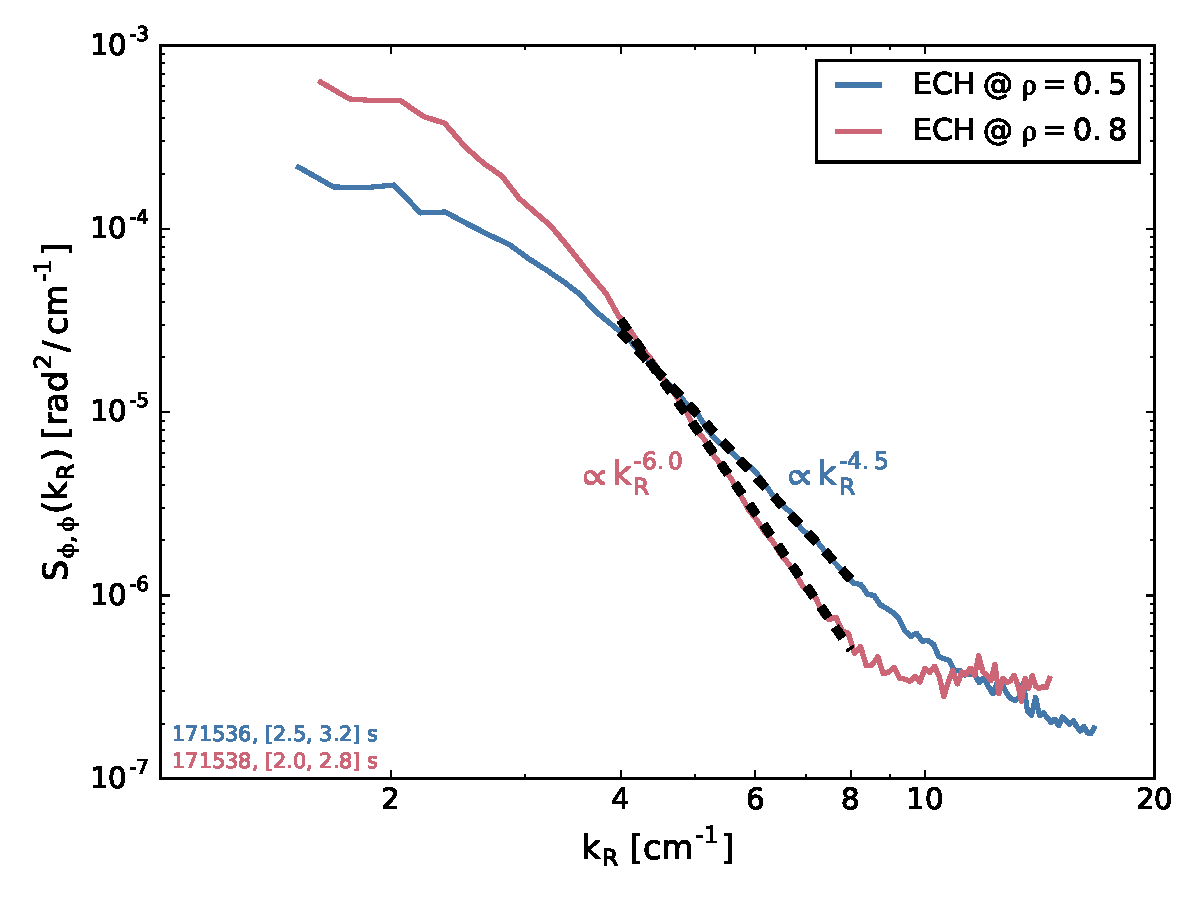
\includegraphics[width = 0.9 \textwidth]{%
    Chapters/TurbulenceMeasurements/figs/Sk_power_law.pdf}
  \caption[PCI frequency-wavenumber spectra]{%
    PCI wavenumber autospectral densities $S_{\phi,\phi}(k)$
    obtained by integrating $S_{\phi,\phi}(k, f)$ in frequency
    between the bounds denoted by the annotating dashed while lines
    in Figure~\ref{fig:TurbulenceMeasurements:Skf_pci}.
    Here, the black dashed lines indicate least-squares power-law fits
    to $S_{\phi,\phi}(k)$.
    The flattening (i.e.\ slower decay) of $S_{\phi,\phi}(k)$
    with $\rhoech = 0.5$ relative to that with $\rhoech = 0.8$
    is reminiscent of results from multiscale gyrokinetic simulations
    in Alcator C-Mod, but
    quantitative comparisons await
    completion of the corresponding multiscale gyrokinetic simulations
    in \diiid.
  }
\label{fig:TurbulenceMeasurements:Sk_power_law}
\end{figure}


\section{TGLF modeling}
\label{sec:TurbulenceMeasurements:Modeling}
To aid the interpretation of the combined PCI-interferometer measurements
described in Section~\ref{sec:TurbulenceMeasurements:Measurements},
linear-stability analysis and quasilinear-transport modeling
were performed with the TGLF code~\footnote{%
  TGLF simulations were graciously performed by Dr. Alessandro Marinoni, but
  the subsequent analysis is the author's own.
}.
Below, Section~\ref{sec:TurbulenceMeasurements:Modeling:TGLF_overview}
provides a brief overview of the TGLF code, and
Section~\ref{sec:TurbulenceMeasurements:Modeling:linear_stability_overview}
presents a global overview
of the TGLF-predicted linear stability
for $\rhoech = 0.5$ to $\rhoech = 0.8$.
In order to facilitate comparisons
between theory and measurement,
Section~\ref{sec:TurbulenceMeasurements:Modeling:wavevectors}
then derives the relationship between
the theoretically relevant field-aligned wavenumber $k_y$ and
the PCI-measured major-radial wavenumber $k_R$.
Next, in an attempt to localize analysis of the TGLF results,
Section~\ref{sec:TurbulenceMeasurements:Modeling:phase_velocity_comparison}
compares the advection of the TGLF-predicted instabilities
by the $\ExB$ velocity
to the PCI-measured phase velocities;
the comparison suggests that
the PCI-measured branch of interest is localized to
$0.6 \leq \rho \leq 0.65$.
Finally, Section~\ref{sec:TurbulenceMeasurements:Modeling:local}
compares the TGLF-predicted electron-density fluctuation spectrum
to the corresponding PCI measurements,
finding qualitative agreement.


\subsection{TGLF overview}
\label{sec:TurbulenceMeasurements:Modeling:TGLF_overview}
TGLF is a gyro-Landau fluid (GLF) model
that captures the dynamics of
both trapped (T) and passing particles
in shaped geometry with finite aspect ratio and $\ExB$ shear
\cite{staebler_pp05, staebler_pp07}.
A GLF model consists of velocity-moment equations
of the gyroaveraged kinetic equation
with moment closures selected
to retain important kinetic effects,
such as Landau damping.
Due to their reduced dimensionality,
GLF models are computationally less expensive
than full gyrokinetic simulations.
TGLF can solve for the linear eigenmodes of
trapped ion and electron modes (TIM and TEM, respectively),
ion and electron temperature gradient (ITG and ETG, respectively) modes,
and kinetic ballooning modes (KBM).
Unfortunately, the default eigenfunction basis
of four Hermite polynomials is typically insufficient
to resolve micro-tearing modes (MTMs)~\cite{staebler_MTM_question}, so
there are no attempts to simulate the MTM in this work.
TGLF additionally uses its eigenmodes
to predict quasilinear transport
using a saturation model fit to results
from nonlinear gyrokinetic simulations~\cite{staebler_pp07},
the most recent of which include
realistic multiscale physics~\cite{staebler_nf17}.


\subsection{Global overview of predicted linear stability}
\label{sec:TurbulenceMeasurements:Modeling:linear_stability_overview}
Using the TGLF\_scan module
in the OMFIT integrated modeling framework~\cite{omfit_nf15},
TGLF simulations were run
to investigate the change in linear stability
when moving from $\rhoech = 0.5$ to $\rhoech = 0.8$.
The simulations span
$0.1 \leq k_y \rho_s \leq 24$ and
$0.3 \leq \rho \leq 0.9$
(only $\rho \gtrsim 0.35$
is accessible to the PCI probe beam, which
propagates vertically through the plasma
at major radius $R = \SI{1.98}{\meter}$).
The equilibrium profiles shown
in Figure~\ref{fig:TurbulenceMeasurements:profiles}
were used as input to TGLF.
Figure~\ref{fig:TurbulenceMeasurements:linear_stability_overview}
displays the resulting linear growth rates $\gamma$ and
plasma-frame phase velocities $\vph = \omega / k_y$
as a function of radial position $\rho$ and
normalized fluctuation wavenumber $k_y \rho_s$.
The predicted change in linear stability
when moving from $\rhoech = 0.5$ to $\rhoech = 0.8$
is largely in accord with intuition
derived from the changes to the normalized inverse scale lengths
shown in Figure~\ref{fig:TurbulenceMeasurements:profiles}(e)-(g).
Perhaps the most substantial change
is that $\rhoech = 0.5$ destabilizes a continuum of
mid-$k$ ($0.5 \lesssim k_y \rho_s \lesssim 5$) electron modes
in the outer region ($\rho \gtrsim 0.6$) of the plasma.
Additionally, in the outer region of the plasma ($\rho \gtrsim 0.6$),
the low-$k$ ion modes ($k_y \rho_s \lesssim 0.3$)
are marginally suppressed and
the high-$k$ electron modes ($k_y \rho_s \gtrsim 10$)
are marginally enhanced
relative to $\rhoech = 0.8$.

\begin{figure}
  \centering
  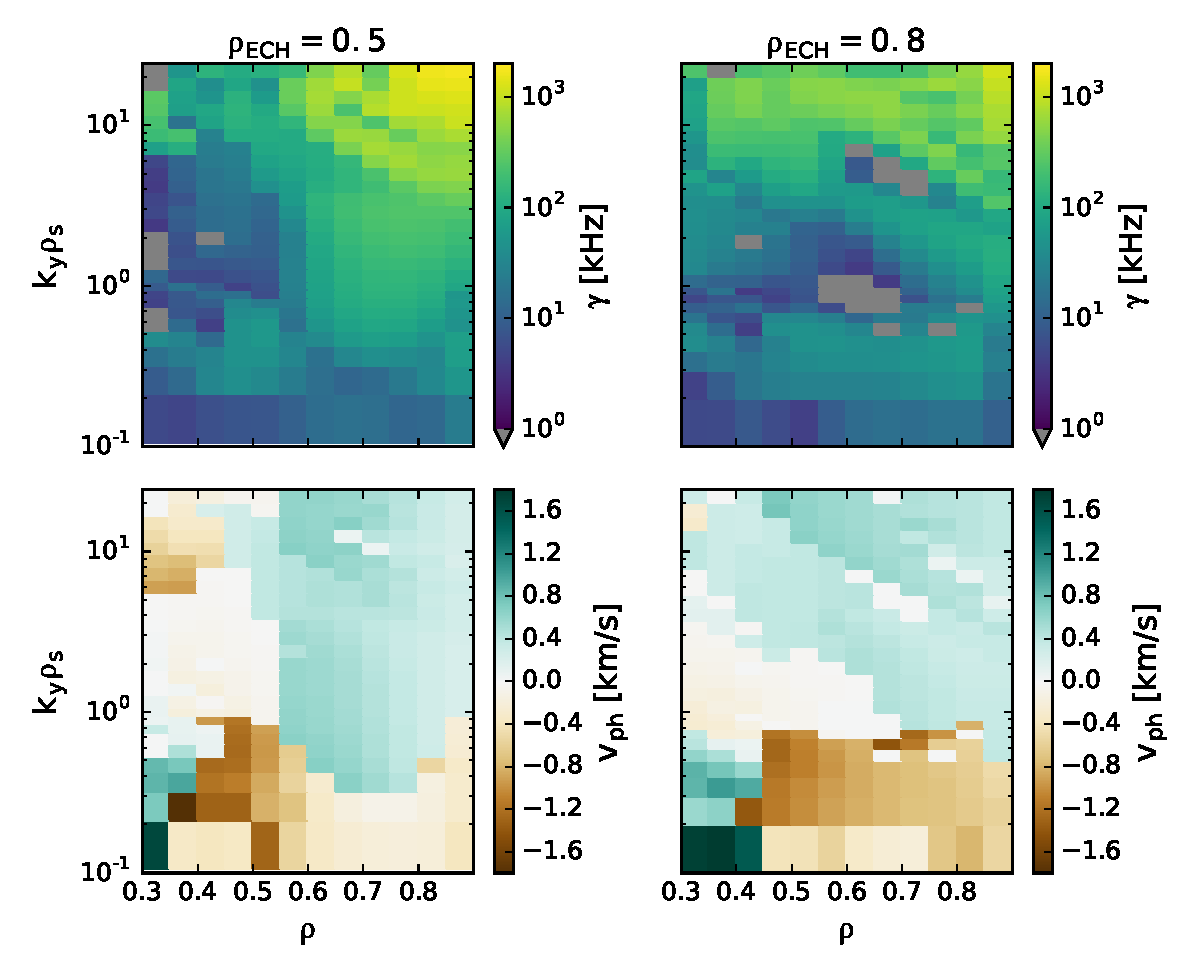
\includegraphics[width = \textwidth]{%
    Chapters/TurbulenceMeasurements/figs/linear_stability_overview.pdf}
  \caption[Global overview of TGLF-predicted linear stability]{%
    Global overview of TGLF-predicted linear stability
    for the profiles shown in
    Figure~\ref{fig:TurbulenceMeasurements:profiles}.
    Linear growth rates $\gamma$ and
    plasma-frame phase velocities $\vph = \omega / k_y$
    are plotted as a function
    of radial position $\rho$ and
    normalized fluctuation wavenumber $k_y \rho_s$
    for $\rhoech = 0.5$ and $\rhoech = 0.8$.
    Electron modes have $\vph > 0$, and
    ion modes have $\vph < 0$.
    The predicted change in linear stability
    when moving from $\rhoech = 0.5$ to $\rhoech = 0.8$
    is largely in accord with intuition
    derived from the changes to the normalized inverse scale lengths
    shown in Figure~\ref{fig:TurbulenceMeasurements:profiles}(e)-(g).
    Growth rates can be compared to
    the $\ExB$ shearing rates $\gamma_E$
    in Figure~\ref{fig:TurbulenceMeasurements:profiles}(h).
  }
\label{fig:TurbulenceMeasurements:linear_stability_overview}
\end{figure}


\subsection{Relation between field-aligned \& PCI-measured wavevectors}
\label{sec:TurbulenceMeasurements:Modeling:wavevectors}
As transport parallel to the magnetic field $\vect{B}$
is much more rapid than transport across the magnetic field,
drift-wave turbulent fluctuations
have a dominant, central wavevector $\vect{k}_0$
that satisfies the field-aligned constraint
$\vect{k}_0 \cdot \vect{B} \approx 0$.
For electrostatic fluctuations,
the magnetic field $\vect{B}$ is well-represented
by the equilibrium field $\Beq$ such that
the field-aligned constraint reduces to
$\vect{k}_0 \cdot \Beq \approx 0$, requiring
\begin{equation}
  \vect{k}_0
  =
  k_{\rho,0} \rhohat
  +
  k_{\theta,0}
  \left[%
    \thetahat
    -
    \left( \frac{B_{\theta,0}}{B_{\zeta,0}} \right) \zetahat
  \right],
  \label{eq:TurbulenceMeasurements:k0}
\end{equation}
where
$k_{\rho,0}$ is the dominant radial wavenumber of the turbulence
(note that velocity shear produces finite $k_{\rho,0}$~\cite{rost_pp14}),
$k_{\theta,0}$ is the dominant poloidal wavenumber of the turbulence,
$B_{\theta,0}$ is the equilibrium poloidal magnetic field,
$B_{\zeta,0}$ is the equilibrium toroidal magnetic field, and
the $(\rho, \theta, \zeta)$ coordinate system
is defined in Figure~\ref{fig:TurbulenceMeasurements:coordinate_geometry}.
Analytic theory and computation are often performed
on field-aligned coordinate systems in which
the $z$-coordinate is along $\Beq$,
the $x$-coordinate is in the radial direction, and
the $y$-coordinate is perpendicular to $\Beq$ but
within a flux surface.
In such a field-aligned coordinate system,
$\vect{k}_0 - k_{\rho,0}\rhohat$
is aligned with the $y$-coordinate
% i.e.\ $\vect{k}_0 = |\vect{k}_0| \hat{\vect{y}}$
such that one is led naturally to define
\begin{equation}
  \vect{k}_y
  =
  k_{\theta,0}
  \left[%
    \thetahat
    -
    \left( \frac{B_{\theta,0}}{B_{\zeta,0}} \right) \zetahat
  \right].
  \label{eq:TurbulenceMeasurements:ky}
\end{equation}
The wavenumber $k_y$ (or its dimensionless equivalent, $k_y \rho_s$)
is an important parameter in the classification and understanding
of turbulent fluctuations.

\begin{figure}
  \centering
  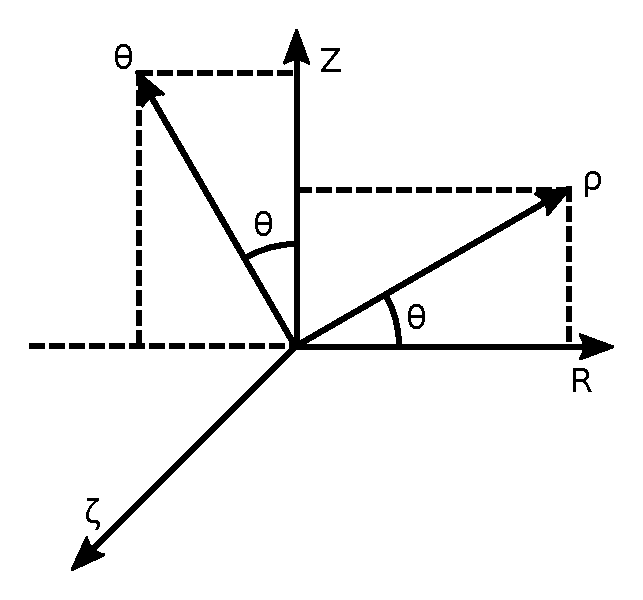
\includegraphics[width = 0.5 \textwidth]{%
    Chapters/TurbulenceMeasurements/figs/coordinate_geometry.pdf}
  \caption[Measurement coordinate system]{%
    Measurement coordinate system.
    Here, $R$ is the major-radial direction,
    $Z$ is the lab-frame vertical direction,
    $\zeta$ is the toroidal angle,
    $\theta$ is the poloidal angle, and
    $\rho$ is a flux-surface label
    corresponding to the square root
    of the normalized toroidal magnetic-field flux.
  }
\label{fig:TurbulenceMeasurements:coordinate_geometry}
\end{figure}

To make contact with theory, then,
it is important to understand the relation between $k_y$ and
the PCI-measured wavevectors.
As a line-integrated measurement,
PCI is sensitive to fluctuations with wavevectors $\kpci$
that are perpendicular to the beam path.
Thus, for the vertical beam path of \diiid's PCI,
\begin{equation}
  \kpci \cdot \Zhat = 0.
  \label{eq:TurbulenceMeasurements:kpci_perp_to_Z}
\end{equation}
As with $\vect{k}_0$, $\kpci$ is also field-aligned
such that (for electrostatic fluctuations)
\begin{equation}
  \kpci \cdot \Beq \approx 0.
  \label{eq:TurbulenceMeasurements:kpci_perp_to_B0}
\end{equation}
In general, $\kpci \neq \vect{k}_0$.
Instead, it is suitable to define
\begin{equation}
  \kpci = \vect{k}_0 + \delta \vect{k}.
  \label{eq:TurbulenceMeasurements:kpci_general}
\end{equation}
The PCI will measure finite signal only if
there exists a $\delta\vect{k}$
within the spatial bandwidth $\Delta\vect{k}$ of the turbulence
such that the resulting $\kpci$ from
(\ref{eq:TurbulenceMeasurements:kpci_general})
satisfies both
(\ref{eq:TurbulenceMeasurements:kpci_perp_to_Z}) and
(\ref{eq:TurbulenceMeasurements:kpci_perp_to_B0}).
(Note that the above reasoning also holds
for any other vertically line-integrated measurement
of field-aligned turbulence,
such as those made by the heterodyne interferometer
constructed in this work).
Decomposing $\delta\vect{k}$
in the $(\rho, \theta, \zeta)$ coordinate system
defined in Figure~\ref{fig:TurbulenceMeasurements:coordinate_geometry}
such that
$\delta\vect{k}
=
\delta k_{\rho} \rhohat
+
\delta k_{\theta} \thetahat
+
\delta k_{\zeta} \zetahat$,
constraint (\ref{eq:TurbulenceMeasurements:kpci_perp_to_Z}) requires
\begin{equation}
  \delta k_{\rho}
  =
  -\delta k_{\rho,0}
  -
  (k_{\theta,0} + \delta k_{\theta}) \cot\theta,
  \label{eq:TurbulenceMeasurements:delta_krho}
\end{equation}
and constraint (\ref{eq:TurbulenceMeasurements:kpci_perp_to_B0}) requires
\begin{equation}
  \delta k_{\zeta}
  =
  -\left( \frac{B_{\theta,0}}{B_{\zeta,0}} \right) \delta k_{\theta}.
  \label{eq:TurbulenceMeasurements:delta_kzeta}
\end{equation}
Using (\ref{eq:TurbulenceMeasurements:delta_krho}) and
(\ref{eq:TurbulenceMeasurements:delta_kzeta}),
$\kpci$ from (\ref{eq:TurbulenceMeasurements:kpci_general}) reduces to
\begin{equation}
  \kpci
  =
  -\left(%
    \frac{k_{\theta,0} + \delta k_{\theta}}{\sin\theta}
  \right)
  \left[%
    \Rhat
    +
    \left( \frac{B_{\theta,0} \sin\theta}{B_{\zeta,0}} \right) \zetahat
  \right],
  \label{eq:TurbulenceMeasurements:kpci_explicit}
\end{equation}
where $\Rhat$ is the unit vector in the major-radial direction and
is related to $\rhohat$ and $\thetahat$
as defined in Figure~\ref{fig:TurbulenceMeasurements:coordinate_geometry}.
Because $|B_{\theta,0}| \ll |B_{\zeta,0}|$,
the PCI is sensitive to fluctuations
with wavevectors that are predominantly in the major-radial direction.
If measurements are made with a one-dimensional detector array,
only a projection of $\kpci$ can be reconstructed.
The one-dimensional detector array of the \diiid\space PCI
is nominally aligned in the major-radial direction
such that the major-radial wavenumber $k_R$ of $\kpci$
can be reconstructed, i.e.\
\begin{equation}
  k_R
  =
  \kpci \cdot \Rhat
  =
  -\left(%
    \frac{k_{\theta,0} + \delta k_{\theta}}{\sin\theta}
  \right)
  \label{eq:TurbulenceMeasurements:kR}.
\end{equation}
In subsequent numerical evaluations,
it is assumed that
$|\delta k_{\theta}| \ll |k_{\theta,0}|$
in order to relate the field-aligned $k_y$ from TGLF
to the PCI-measured major radial wavenumber $k_R$.
Figure~\ref{fig:TurbulenceMeasurements:wavenumber_conversion}
displays profiles of $|k_y \rho_s|$ for various $k_R$ of interest.

\begin{figure}
  \centering
  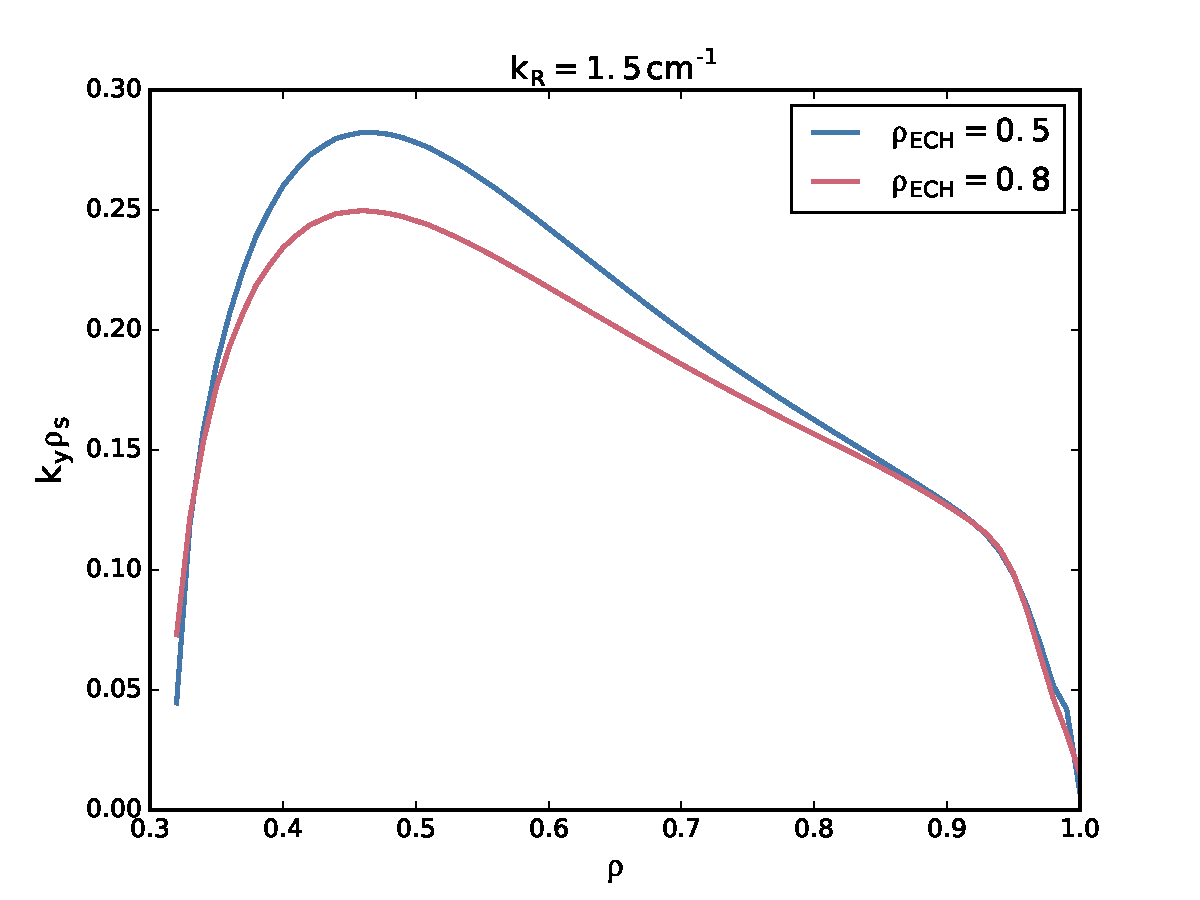
\includegraphics[width = \textwidth]{%
    Chapters/TurbulenceMeasurements/figs/wavenumber_conversion.pdf}
  \caption[Profiles of $k_y \rho_s$ for $k_R = \SI{1.5}{\per\centi\meter}$]{%
    Profiles of $|k_y \rho_s|$ vs.\ radial coordinate $\rho$ for
    the PCI low-$k$ cutoff $k_R = \SI{1.5}{\per\centi\meter}$,
    the interferometer high-$k$ cutoff $k_R = \SI{5}{\per\centi\meter}$, and
    the PCI high-$k$ cutoff $k_R = \SI{25}{\per\centi\meter}$
    in the $\rhoech = 0.5$ and $\rhoech = 0.8$ discharges
    shown in Figure~\ref{fig:TurbulenceMeasurements:profiles}.
    The gray region $(\rho \lesssim 0.35)$
    is inaccessible to the PCI probe beam,
    which propagates vertically through the plasma
    at major radius $R = \SI{1.98}{\meter}$.
    The roll-off in $|ky \rho_s|$ for $\rho \lesssim 0.4$
    is attributable to the $\sin\theta$ major-radial projection, while
    the roll-off for $\rho \gtrsim 0.95$
    is attributable to the edge pedestal.
  }
\label{fig:TurbulenceMeasurements:wavenumber_conversion}
\end{figure}


\subsection{Comparison to PCI-measured phase velocities}
\label{sec:TurbulenceMeasurements:Modeling:phase_velocity_comparison}
In an attempt to localize analysis of the TGLF results,
the advection of the TGLF-predicted instabilities by the $\ExB$ velocity
can be compared to the PCI-measured phase velocities.
The PCI-measured phase velocity is
\begin{equation}
  \vphpci
  =
  \frac{\omegapci}{k_R}
  =
  \frac{\kpci \cdot \vect{v}}{k_R},
  \label{eq:TurbulenceMeasurements:vphpci_general}
\end{equation}
where $\omegapci$ is the PCI-measured angular frequency,
$\kpci$ is the wavevector (\ref{eq:TurbulenceMeasurements:kpci_explicit}),
$\vect{v}$ is the lab-frame velocity of the fluctuation, and
$k_R$ is the reconstructed major-radial wavenumber
(\ref{eq:TurbulenceMeasurements:kR}).
By field-aligned constraint
(\ref{eq:TurbulenceMeasurements:kpci_perp_to_B0}),
$\kpci \cdot \vect{v} = \kpci \cdot \vperp$, where
$\vperp$ is the velocity
perpendicular to the equilibrium magnetic field.
The perpendicular velocity $\vperp$ is simply the sum of
the $\ExB$ velocity $\vExB$ and
the plasma-frame phase velocity
$\vect{v}_{\text{ph}}^{\text{plasma}}$ of the fluctuation;
here, the plasma-frame phase velocity is approximated
by that of the dominant wavevector, i.e.\
$\vect{v}_{\text{ph}}^{\text{plasma}} \approx \vphplasma \kzerohat$,
where $\kzerohat = \vect{k}_0 / |\vect{k}_0|$ and
$\vect{k}_0$ is the dominant wavevector defined in
(\ref{eq:TurbulenceMeasurements:k0}).
Thus, $\vperp \approx \vExB + \vphplasma \kzerohat$, and
\begin{equation}
  \omegapci
  =
  \kpci \cdot \vperp
  \approx
  \kpci \cdot \vExB
  +
  (\kpci \cdot \kzerohat)
  \vphplasma.
  \label{eq:TurbulenceMeasurements:omegapci}
\end{equation}
Now, the electrostatic potential $\varphi = \varphi(\rho)$
is a flux function such that
the corresponding electric field is
$\vect{E} = -\nabla \varphi = E_r(\rho, \theta) \rhohat$.
The resulting $\ExB$ velocity is
\begin{align}
  \vExB
  =
  \frac{\vect{E} \times \Beq}{B_0^2}
  % \notag \\
  =
  \frac{E_r(\rho, \theta)}{B_0^2}
  \left(%
    B_{\theta} \zetahat
    -
    B_{\zeta} \thetahat
  \right).
  \label{eq:TurbulenceMeasurements:vExB}
\end{align}
Using
$\kpci$ from (\ref{eq:TurbulenceMeasurements:kpci_explicit}),
$\vExB$ from (\ref{eq:TurbulenceMeasurements:vExB}),
$\vect{k}_0$ from (\ref{eq:TurbulenceMeasurements:k0}),
$\omegapci$ from (\ref{eq:TurbulenceMeasurements:omegapci}),
$k_R$ from (\ref{eq:TurbulenceMeasurements:kR}), and
a bit of algebra,
the PCI-measured phase velocity
(\ref{eq:TurbulenceMeasurements:vphpci_general})
readily reduces to
\begin{equation}
  \vphpci
  =
  \left[%
    \frac{E_r(\rho, \theta)}{B_0}
    -
    \vphplasma
  \right]
  \left( \frac{B_0}{B_{\zeta,0}} \right)
  \sin\theta.
  \label{eq:TurbulenceMeasurements:vphpci}
\end{equation}
The sign convention for the plasma-frame phase velocity is such that
$\vphplasma > 0$ for electron modes and
$\vphplasma < 0$ for ion modes.
For physical intuition regarding this sign convention,
consider a region of the plasma with $E_r > 0$;
here, electron modes propagate against the $\ExB$ direction
(decreasing $\vphpci$ relative to the $\ExB$ contribution alone), and
ion modes propagate in the $\ExB$ direction
(increasing $\vphpci$ relative to the $\ExB$ contribution alone).
The $B_0 / B_{\zeta,0}$ multiplicative enhancement to $\vphpci$
results from $|k_R| < |\kpci|$
when the magnetic field is not solely toroidal, and
the $\sin\theta$ term
provides the major-radial projection
required by the constraint
(\ref{eq:TurbulenceMeasurements:kpci_perp_to_Z});
note that $\vphpci$ changes sign about the midplane ($\theta = 0$)
due to this major-radial projection.
As the spatially filtering mask
\cite{dorris_rsi09, dorris_phd}
was not used in this experiment,
the PCI measurements cannot be localized
to above or below the midplane, and
only the magnitude of $\vphpci$ will be considered here.
Figure~\ref{fig:TurbulenceMeasurements:predicted_pci_phase_velocities}
compares the magnitude of the predicted PCI phase velocity
from (\ref{eq:TurbulenceMeasurements:vphpci})
to the measured PCI phase velocities
from the annotated turbulent branches
in Figure~\ref{fig:TurbulenceMeasurements:Skf_pci} and
infers that this turbulence is localized to
$0.6 \leq \rho \leq 0.65$.

\begin{figure}
  \centering
  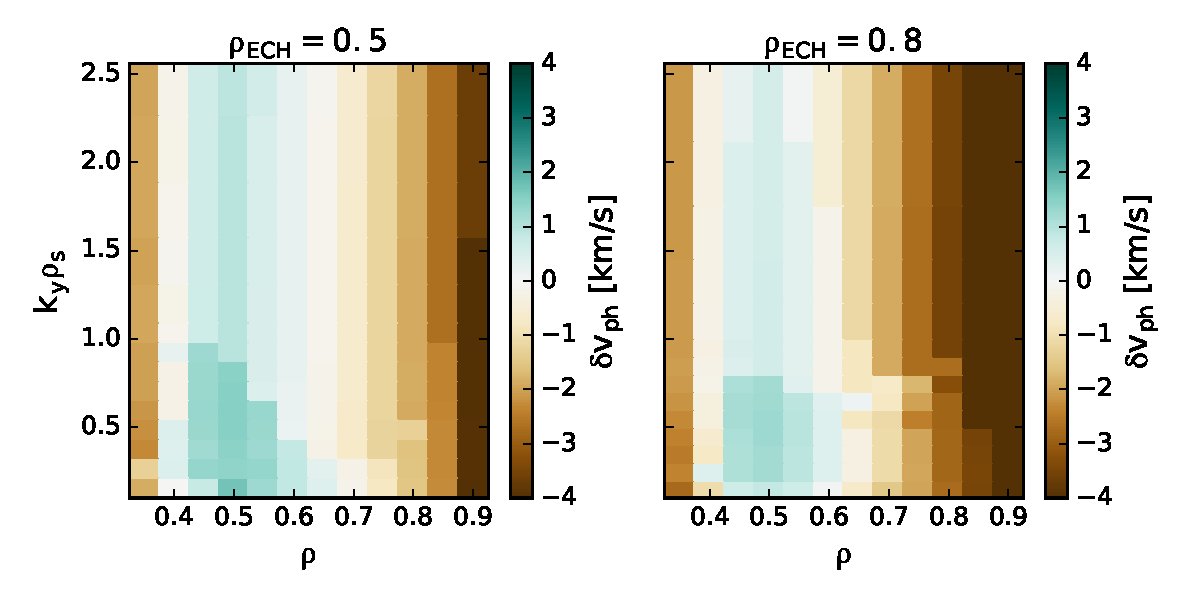
\includegraphics[width = \textwidth]{%
    Chapters/TurbulenceMeasurements/figs/predicted_pci_phase_velocities.pdf}
  \caption[Comparison of predicted and measured PCI phase velocities]{%
    Comparison of predicted and measured PCI phase velocities.
    Here, $\delta \vph$ is the difference between
    the predicted phase velocity and
    the measured phase velocity.
    The predicted phase velocity
    (\ref{eq:TurbulenceMeasurements:vphpci})
    is computed using
    the equilibrium profiles shown in
    Figure~\ref{fig:TurbulenceMeasurements:profiles} and
    the TGLF-predicted plasma-frame phase velocites shown in
    Figure~\ref{fig:TurbulenceMeasurements:linear_stability_overview}.
    The measured phase velocities correspond
    to the annotated turbulent branches in
    Figure~\ref{fig:TurbulenceMeasurements:Skf_pci}.
    The wavenumber range $k_y \rho_s$ considered here
    is restricted to $k_R \leq \SI{15}{\per\centi\meter}$,
    the maximum PCI-measured wavenumber in
    Fig~\ref{fig:TurbulenceMeasurements:Skf_pci}.
    The minimum discrepancy between
    the predicted and measured PCI phase velocities
    occurs between at $0.6 \leq \rho \leq 0.65$,
    suggesting that the annotated turbulent branches in
    Figure~\ref{fig:TurbulenceMeasurements:Skf_pci}
    are localized to $0.6 \leq \rho \leq 0.65$.
  }
\label{fig:TurbulenceMeasurements:predicted_pci_phase_velocities}
\end{figure}

As a brief aside, it should be emphasized
that the radial electric field $E_r$
in (\ref{eq:TurbulenceMeasurements:vphpci})
is \emph{not} a flux function.
To see this, recall that
the corresponding electrostatic potential
\emph{is} a flux function,
i.e.\ $\varphi = \varphi(\rho) = \varphi(\psi)$,
where $\psi$ is the flux-surface label
corresponding to the poloidal magnetic-field flux per radian.
Now,
\begin{align}
  E_r(\rho, \theta)
  &=
  -\left( \frac{\partial\varphi}{\partial r} \right)
  \notag \\
  &=
  -\left( \frac{d\varphi}{d\psi} \right)
  \left( \frac{\partial\psi}{\partial r} \right)
  \notag \\
  &=
  -\left( \frac{d\varphi}{d\psi} \right)
  \left( R B_{\theta} \right),
\end{align}
where the last line follows from the definition
of $\psi$ as the poloidal magnetic-field flux per radian.
The derivative $d\varphi / d\psi$
is a flux function because $\varphi$ is a flux function, and
this implies that $E_r / (R B_{\theta})$ is also a flux function.
Thus, the radial electric field at any point
within the last closed flux surface can be computed
from the radial electric field
along the outboard midplane (where $\theta = 0$) as follows
\begin{equation}
  \left.
  \frac{E_r}{R B_{\theta}}
  \right|_{\rho, \theta}
  =
  \left.
  \frac{E_r}{R B_{\theta}}
  \right|_{\rho, \theta = 0}.
  \label{eq:TurbulenceMeasurements:radial_electric_field}
\end{equation}


\subsection{Quantitative local results}
\label{sec:TurbulenceMeasurements:Modeling:local}
A global overview of the TGLF-predicted linear stability was presented in
Section~\ref{sec:TurbulenceMeasurements:Modeling:linear_stability_overview}.
In Section~\ref{sec:TurbulenceMeasurements:Modeling:phase_velocity_comparison},
the annotated turbulent branches
from Figure~\ref{fig:TurbulenceMeasurements:Skf_pci}
were localized to $0.6 \leq \rho \leq 0.65$.
Thus, it is now reasonable
to perform a more quantitative assessment
of the corresponding local TGLF predictions.
Below, TGLF predictions are shown for $\rho = 0.6$, but
comparable predictions are made at $\rho = 0.65$.

Figure~\ref{fig:TurbulenceMeasurements:linear_stability_local}
displays the TGLF-predicted linear stability
at radial location $\rho = 0.6$
for $\rhoech = 0.5$ and $\rhoech = 0.8$.
Both operational scenarios are predicted
to destabilize ion and electron modes
across multiple spatiotemporal scales, but
$\rhoech = 0.5$ is predicted
to destabilize a continuum
of mid-$k$ ($0.5 \lesssim k_y \rho_s \lesssim 5$) electron modes
that bridge the gap between
low-$k$ ($k_y \rho_s \lesssim 0.5$) ion modes and
high-$k$ ($k_y \rho_s \gtrsim 5$) electron modes,
potentially facilitating cross-scale coupling.
Further, relative to $\rhoech = 0.8$,
the $\rhoech = 0.5$ ion-mode growth rates
are substantially reduced
(becoming comparable to the $\ExB$ shearing rate
shown in Figure~\ref{fig:TurbulenceMeasurements:profiles}(h)), and
the high-$k$ electron-mode growth rates
are marginally enhanced,
both of which may also facilitate cross-scale coupling.

\begin{figure}
  \centering
  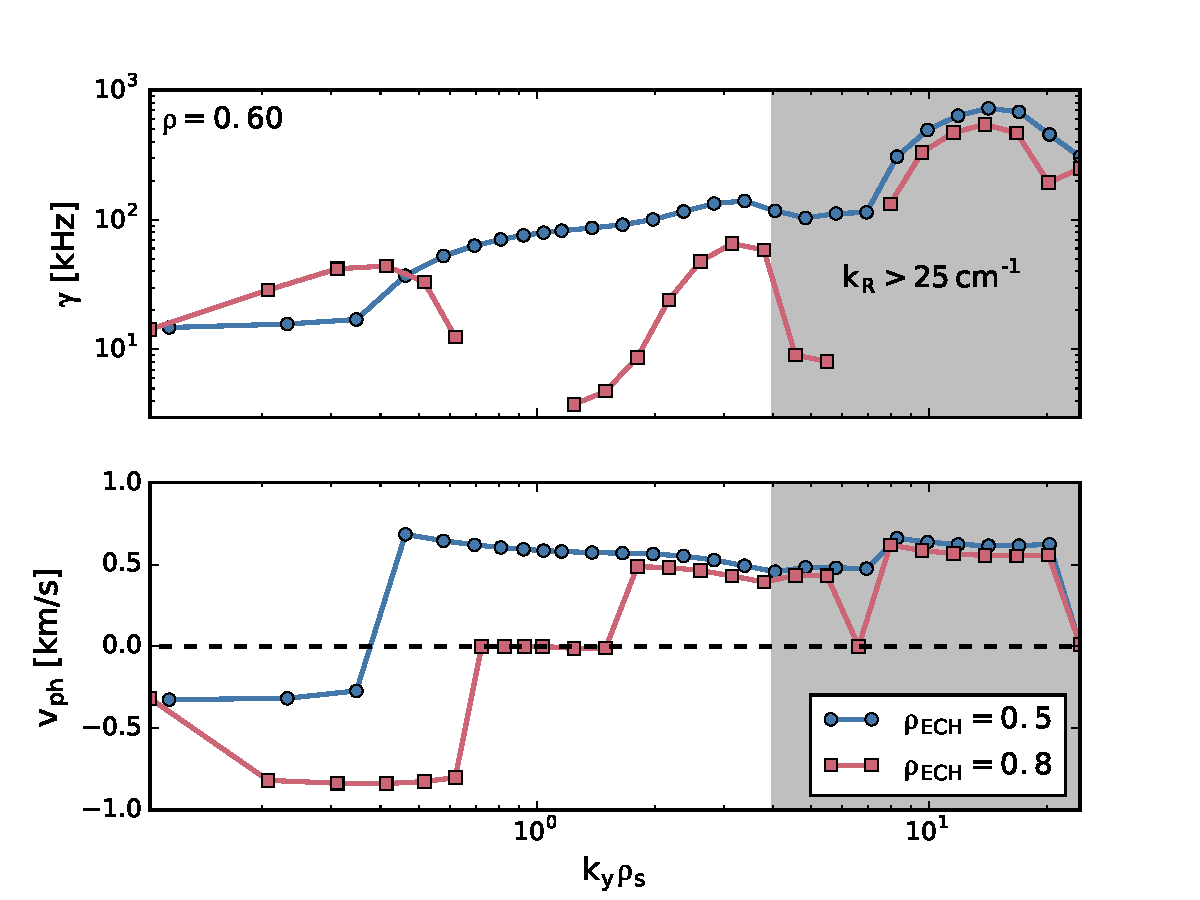
\includegraphics[width = \textwidth]{%
    Chapters/TurbulenceMeasurements/figs/linear_stability_local.pdf}
  \caption[TGLF-predicted linear stability at $\rho = 0.6$]{%
    TGLF-predicted linear stability at $\rho = 0.6$
    for the profiles shown in
    Figure~\ref{fig:TurbulenceMeasurements:profiles}.
    Linear growth rates $\gamma$ and
    plasma-frame phase velocities $\vph = \omega / k_y$
    are plotted as a function of
    normalized fluctuation wavenumber $k_y \rho_s$
    for $\rhoech = 0.5$ and $\rhoech = 0.8$.
    Electron modes have $\vph > 0$, and
    ion modes have $\vph < 0$.
    The gray region exceeds the spatial bandwidth
    of the combined PCI-interferometer
    developed in this work.
    Growth rates can be compared
    to the $\ExB$ shearing rates $\gamma_E$
    in Figure~\ref{fig:TurbulenceMeasurements:profiles}(h).
  }
\label{fig:TurbulenceMeasurements:linear_stability_local}
\end{figure}

Howard \emph{et al.} suggest a linear-stability ``rule of thumb''
for gauging the importance of cross-scale coupling~\cite{howard_pp16}.
The rule of thumb attempts to quantify the relative ``strength''
of electron-scale to ion-scale turbulence
by examining the ratio of
the maximum electron-scale growth rate $\gammahighk$ to
the maximum ion-scale growth rate $\gammalowk$,
with larger values of $\gammahighk / \gammalowk$
corresponding to increased cross-scale coupling.
Howard \emph{et al.} constrain their search
for $\gammahighk$ to $2 \leq k_y \rho_s \leq 48$ and
for $\gammalowk$ to $0.25 \leq k_y \rho_s \leq 0.75$.
For consistency, this same selection criterion is used below.
For $\rhoech = 0.8$,
Figure~\ref{fig:TurbulenceMeasurements:linear_stability_local} shows that
$\gammahighk = \SI{540}{\kilo\hertz}$ at $k_y \rho_s = 14$ and
$\gammalowk = \SI{43}{\kilo\hertz}$ at $k_y \rho_s = 0.4$ such that
$\gammahighk / \gammalowk = 12.6$;
with such a small value,
the rule of thumb suggests that cross-scale coupling
is insignificant.
For $\rhoech = 0.5$,
Figure~\ref{fig:TurbulenceMeasurements:linear_stability_local} shows that
$\gammahighk = \SI{720}{\kilo\hertz}$ at $k_y \rho_s = 14$ and
$\gammalowk = \SI{63}{\kilo\hertz}$ at $k_y \rho_s = 0.7$ such that
$\gammahighk / \gammalowk = 11.4$,
less than the $\rhoech = 0.8$ case.
It should be noted, however,
that the distinct mid-$k$ electron branch
in Figure~\ref{fig:TurbulenceMeasurements:linear_stability_local}
is \emph{absent} from the plasmas
used to develop the rule of thumb;
further, the above $\gammalowk$ for $\rhoech = 0.5$
corresponds to this mid-$k$ electron branch.
If $\gammalowk$ is instead restricted to an ion mode,
$\gammalowk = \SI{17}{\kilo\hertz}$ at $k_y \rho_s = 0.35$ such that
$\gammahighk / \gammalowk = 42$;
cross-scale coupling can be important in ELMy H-mode plasmas
with this $\gammahighk / \gammalowk$~\cite{howard_ppcf18}.

In addition to assessing linear stability,
TGLF can predict the electron-density fluctuation spectrum
using quasilinear transport and
a model for the nonlinear saturation of the turbulence.
This saturation model is fit to results
from nonlinear gyrokinetic simulations~\cite{staebler_pp07},
the most recent of which include
realistic multiscale physics~\cite{staebler_nf17}.
The multiscale saturation model is referred to as SAT$1$.
The density fluctuation spectrum
predicted by TGLF-SAT$1$ at $\rho = 0.6$
is shown Figure~\ref{fig:TurbulenceMeasurements:density_spectra_local}.
Within the PCI sensitivity and wavenumber domain,
the predicted spectra are qualitatively consistent
with the PCI-measured spectra
in Figure~\ref{fig:TurbulenceMeasurements:Sk_power_law}.
Specifically, the $\rhoech = 0.5$ spectrum
is noticeably flatter (i.e.\ decays more slowly)
than the $\rhoech = 0.8$ spectrum, which
may be indicative of enhanced cross-scale coupling~\cite{howard_pp16}.
Further, the intersection of the two predicted spectra
is in rough agreement
with that observed in the PCI-measured spectra.
However, the predicted and measured power laws
quantitatively disagree.
It should be emphasized that the TGLF-SAT$1$ model
is fit to just a handful~\cite{staebler_nf17}
of realistic multiscale gyrokinetic simulations
corresponding to Alcator C-Mod L-mode plasmas, so
quantitative agreement may improve
when additional multiscale simulations are completed and
the TGLF-SAT$1$ model is recalibrated.

\begin{figure}
  \centering
  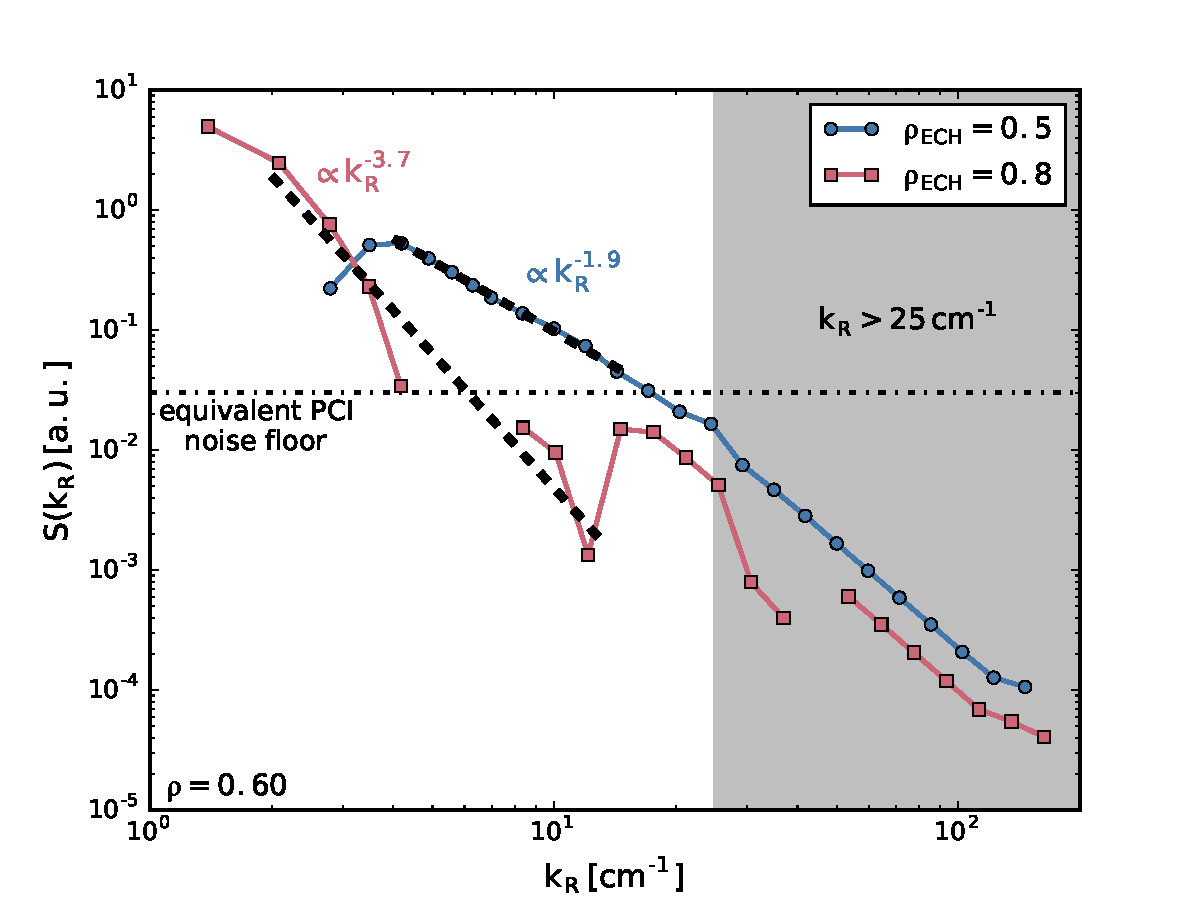
\includegraphics[width = \textwidth]{%
    Chapters/TurbulenceMeasurements/figs/density_spectra_local.pdf}
  \caption[TGLF-predicted electron-density fluctuation spectra]{%
    Electron-density fluctuation spectra
    predicted by TGLF-SAT$1$
    at radial location $\rho = 0.6$
    for $\rhoech = 0.5$ and $\rhoech = 0.8$.
    The gray region exceeds the spatial bandwidth
    of the combined PCI-interferometer
    developed in this work.
    The equivalent PCI noise floor,
    indicated by the horizontal dash-dot line,
    is inferred from the noise floor
    in Figure~\ref{fig:TurbulenceMeasurements:Sk_power_law};
    that is, for $\rhoech = 0.5$
    the equivalent noise floor intersects $S(k_R)$
    at $k_R \approx \SI{15}{\per\centi\meter}$,
    which is roughly equivalent to the $\rhoech = 0.5$ noise floor
    in Figure~\ref{fig:TurbulenceMeasurements:Sk_power_law}.
    Within the PCI sensitivity and wavenumber domain,
    the predicted spectra are qualitatively consistent
    with the PCI-measured spectra
    in Figure~\ref{fig:TurbulenceMeasurements:Sk_power_law}.
    The black dashed lines indicate least-squares power-law fits
    to the predicted $S(k_R)$;
    the resulting power laws quantitatively disagree
    with the PCI-measured power laws in
    Figure~\ref{fig:TurbulenceMeasurements:Sk_power_law}.
  }
\label{fig:TurbulenceMeasurements:density_spectra_local}
\end{figure}


\bibliographystyle{plainurl}
\bibliography{references}
